\section{GPIO}

\subsection{Mit Dokumentation arbeiten}
\subsubsection{Pinout}
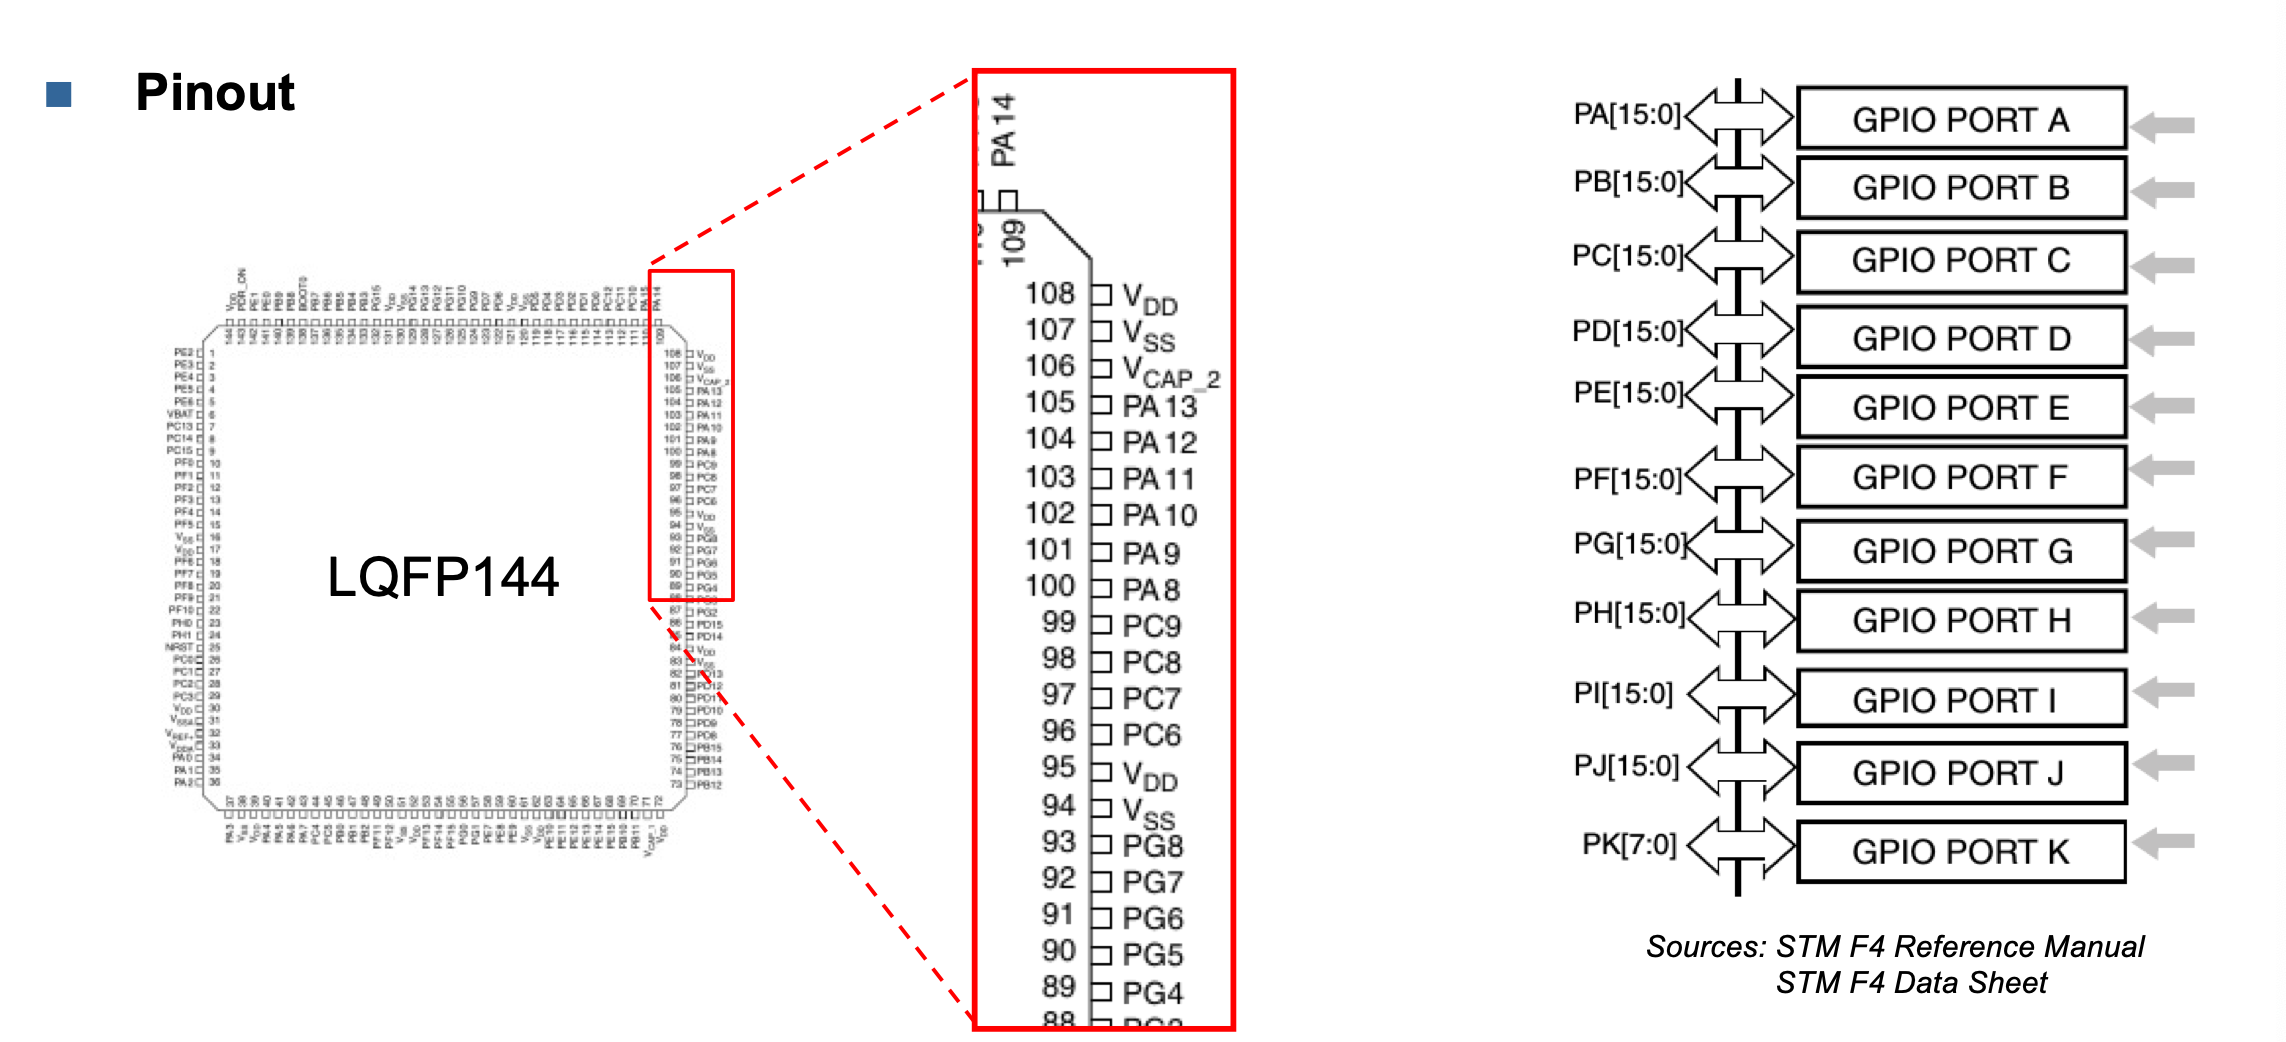
\includegraphics[width=0.3\textwidth]{sections/images/pinout.png}

\subsubsection{Register}
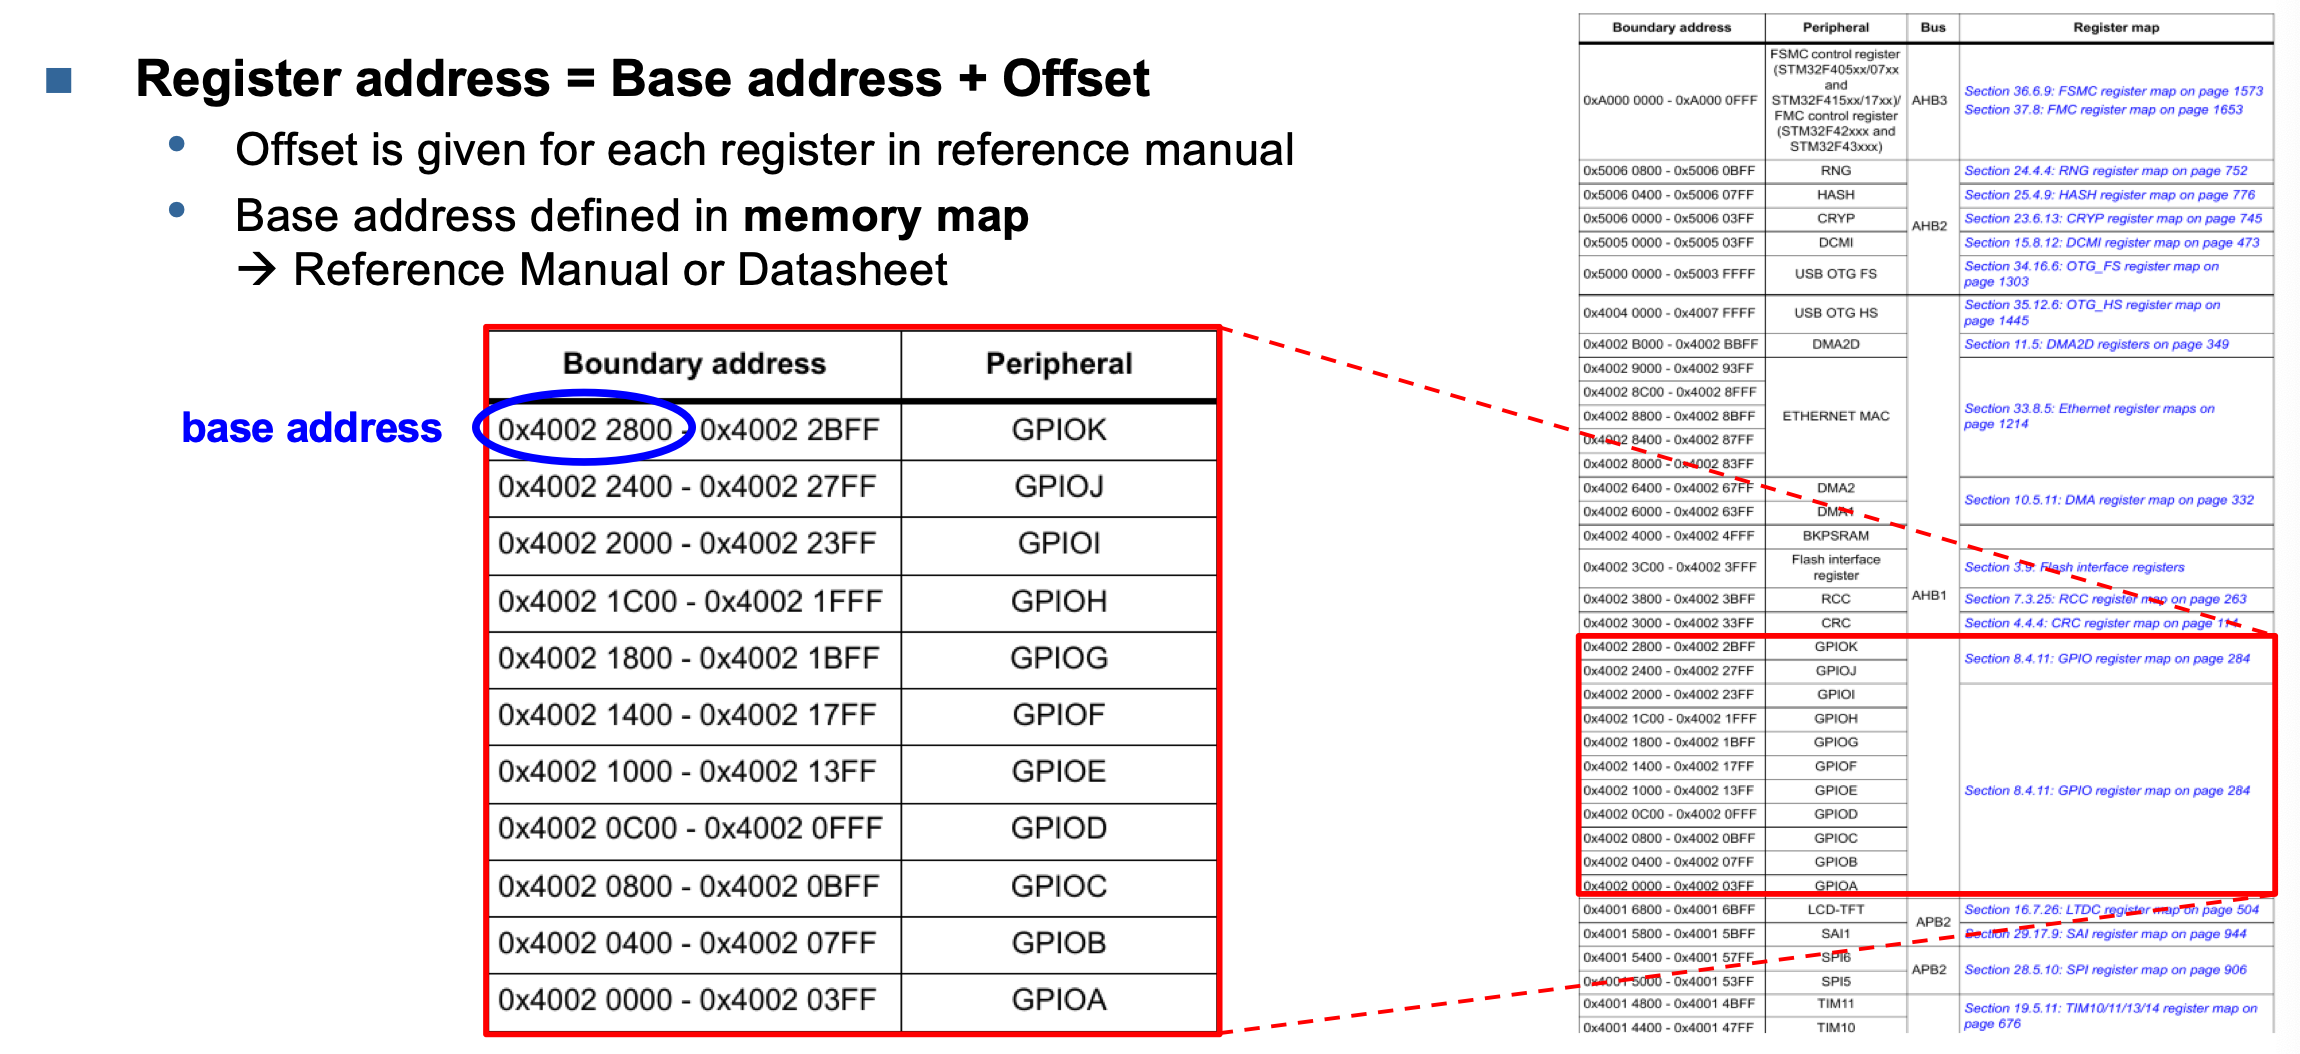
\includegraphics[width=0.3\textwidth]{sections/images/register.png}

\subsection{Konzept und Implementierung von GPIO}
\subsubsection{Konzept}
\begin{itemize}
    \item GPIO addressiert das Problem, dass die CPU nicht genügend I/O Pins hat.
    \item GPIO ist ein Interface zwischen CPU und Peripherie.
    \item Die Pins sind konfigurierbar, man kann die gewünschte Funktion wählen.
    \item "Pin Sharing" ist möglich, d.h. ein Pin kann mehrere Funktionen haben.
    \item Ein Output Multiplexer wählt die Funktion des Pins.
    \item Das führt dazu, dass nicht alle Funktionen gleichzeitig verfügbar sind.
    \item Die Pin Konfiguration wird in der Regel statisch festgelegt.
\end{itemize}

\subsubsection{Implementierung STM32F4}
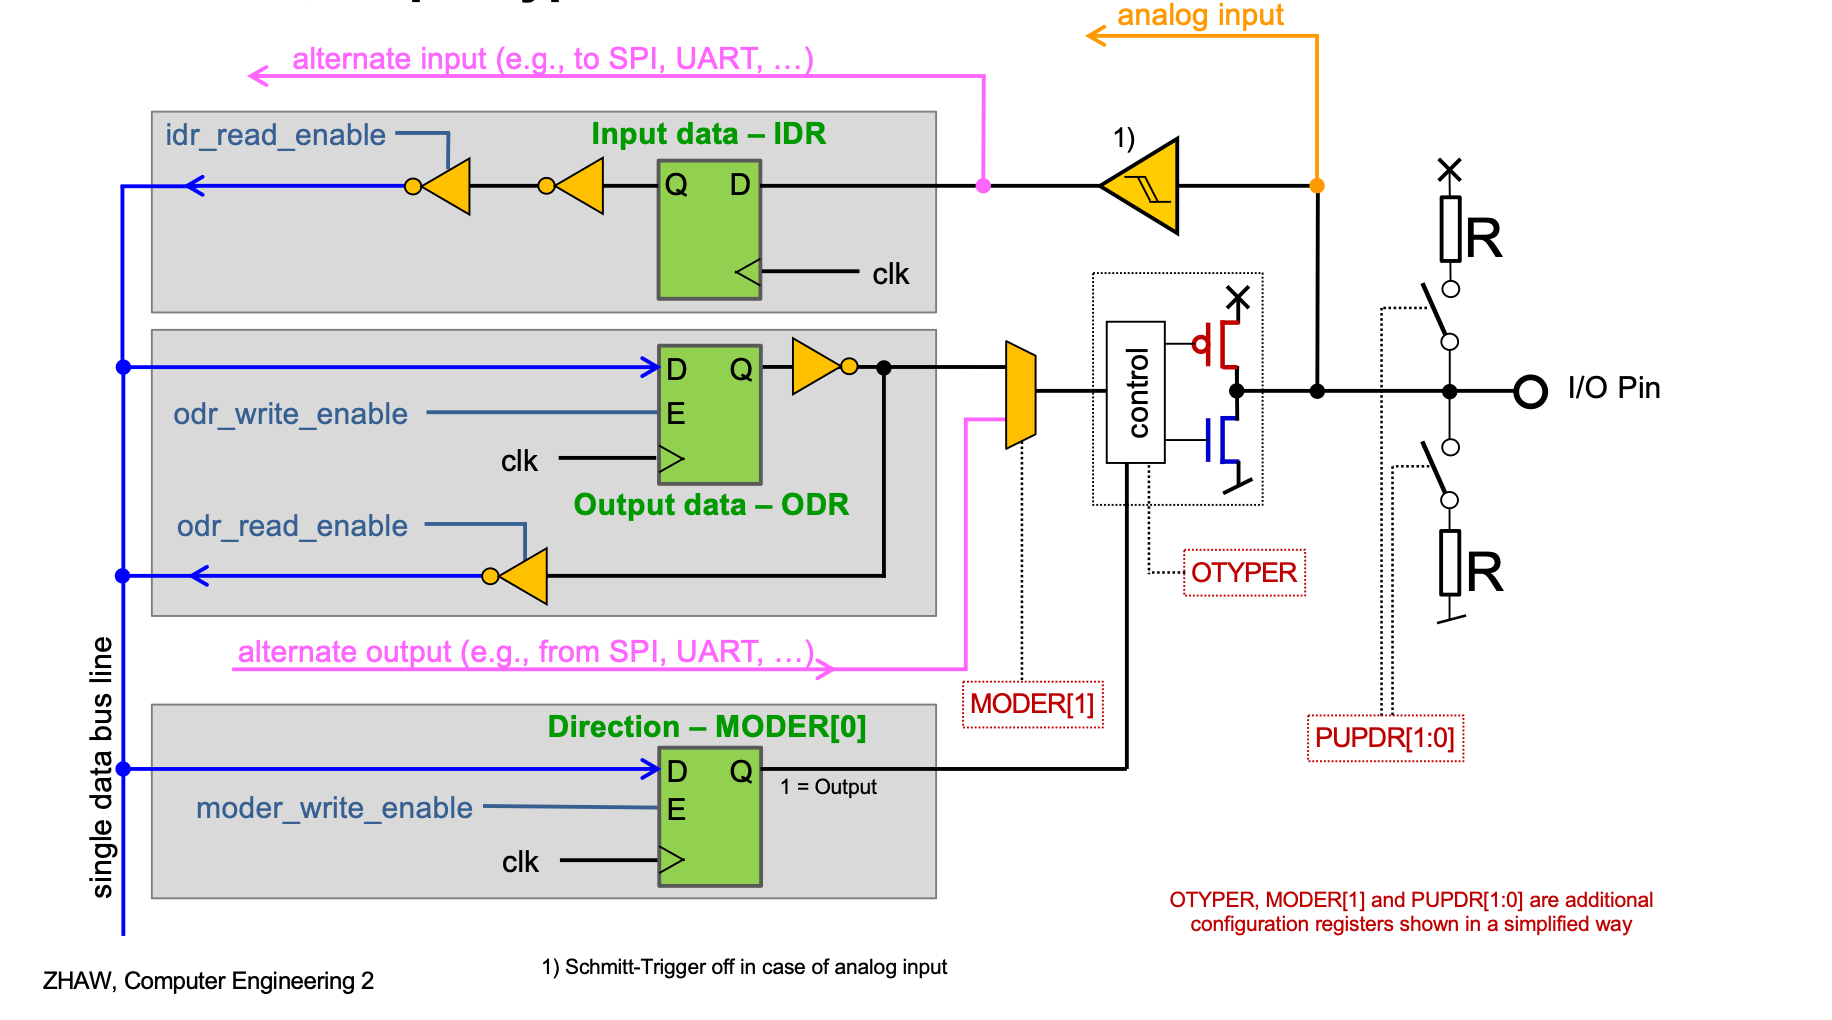
\includegraphics[width=0.3\textwidth]{sections/images/gpio.png}

\subsubsection{Mode Register (Direction)}
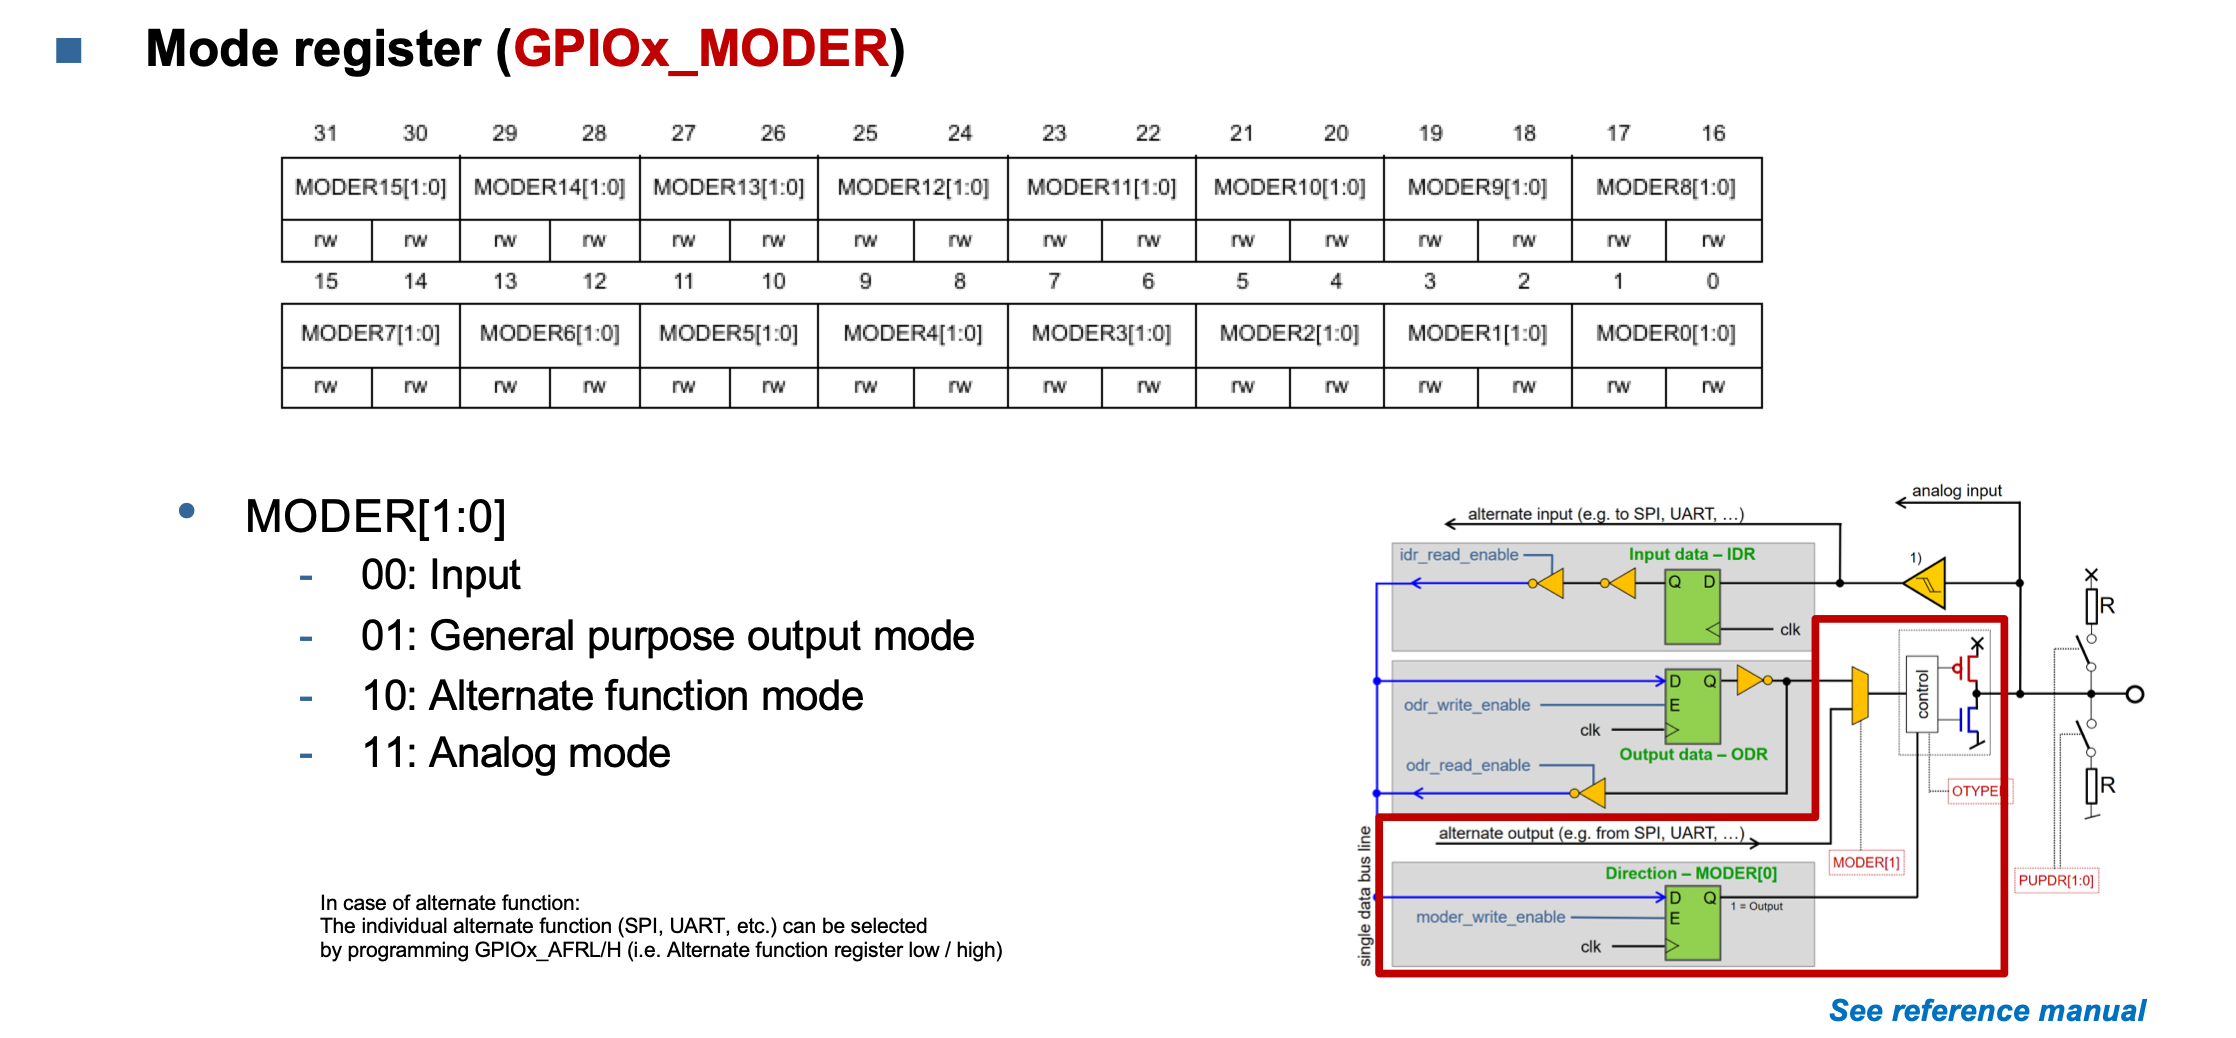
\includegraphics[width=0.3\textwidth]{sections/images/mode_register.png}

\subsubsection{Output Type Register}
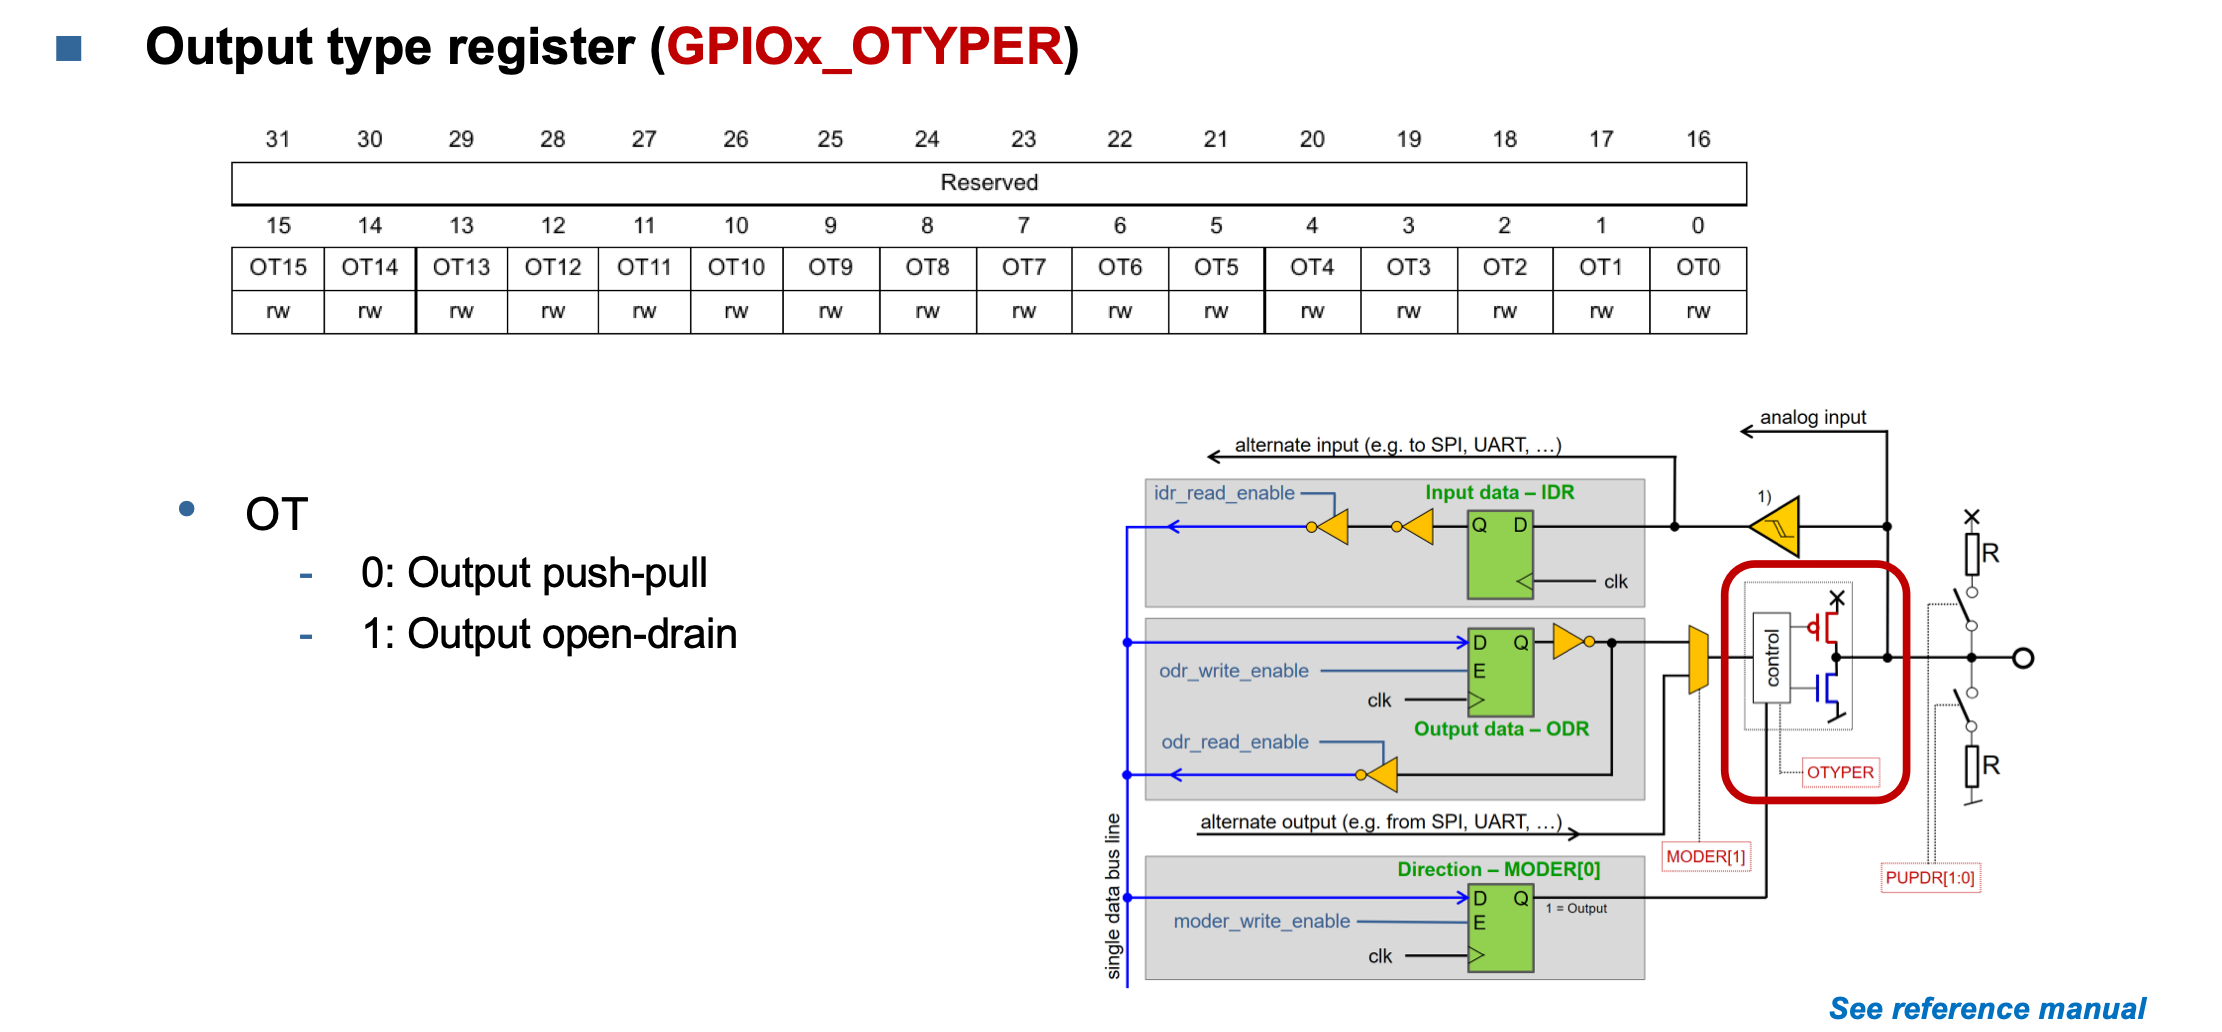
\includegraphics[width=0.3\textwidth]{sections/images/out_type.png}

\subsection{Push-Pull vs. Open-Drain}
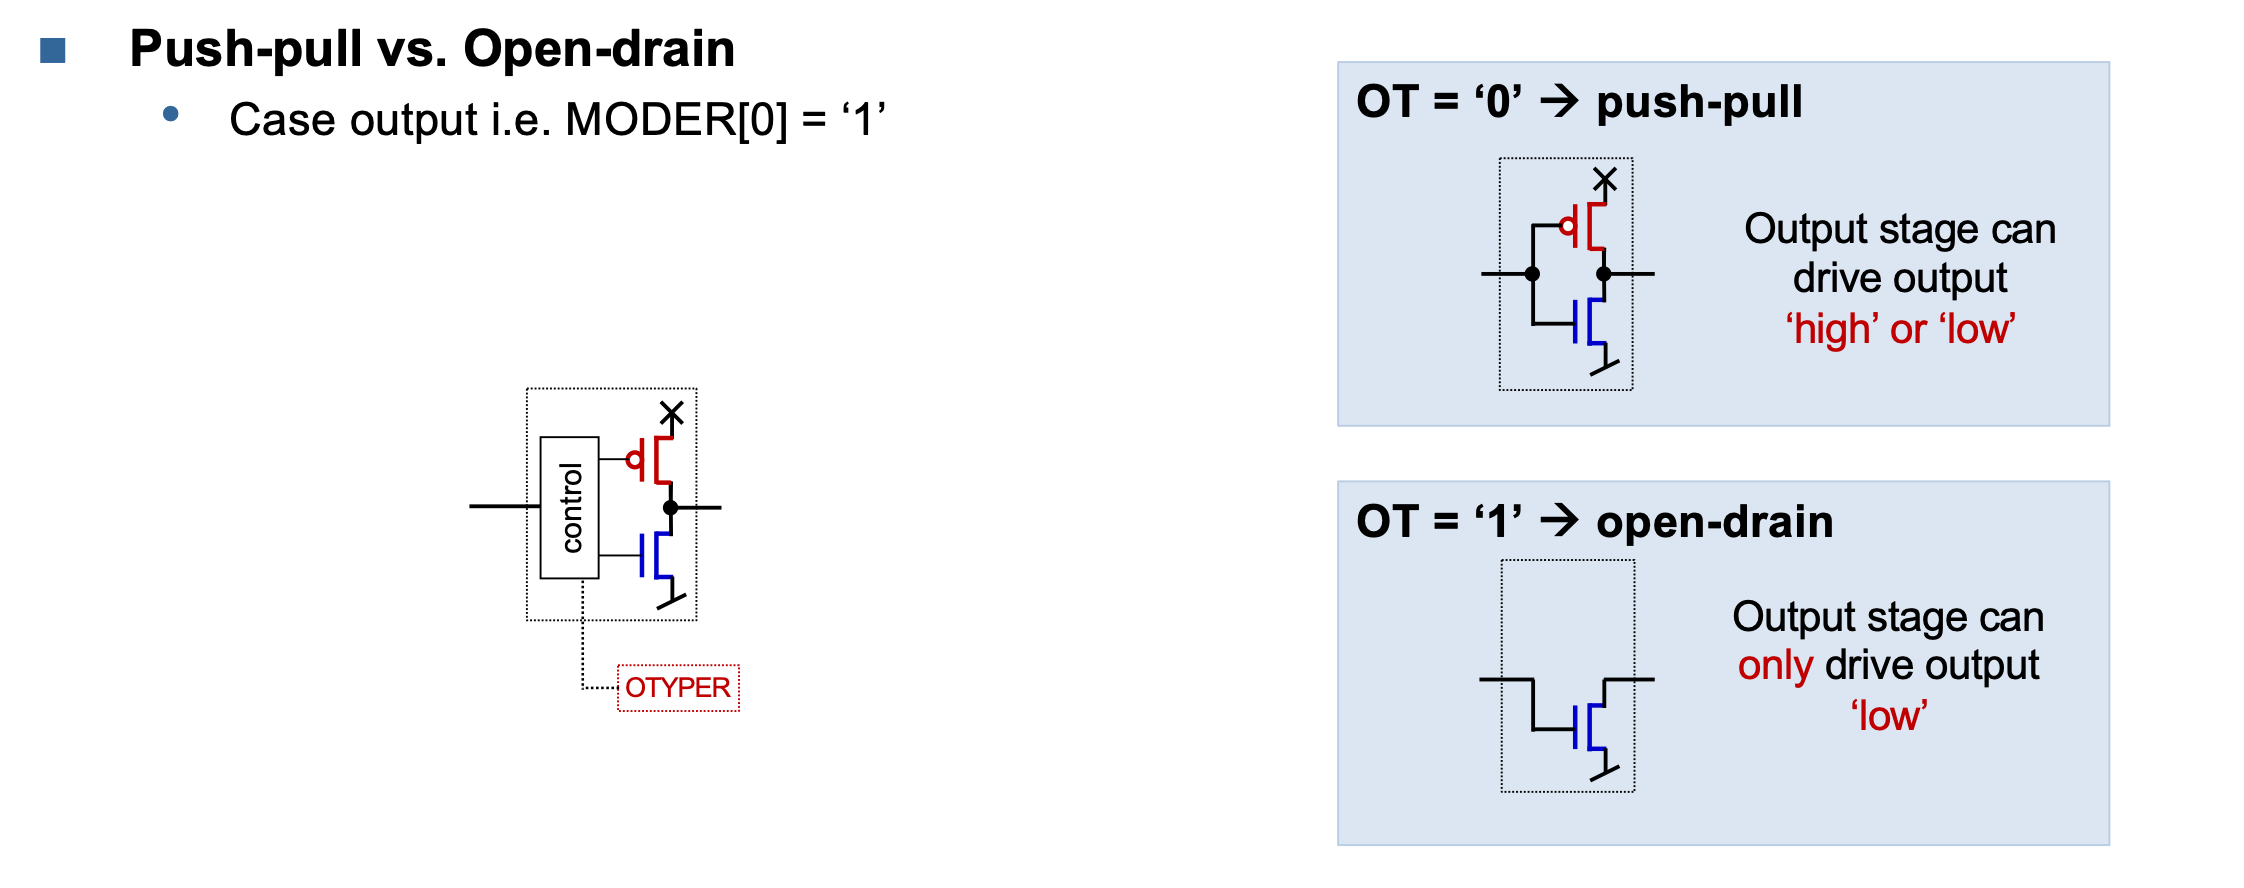
\includegraphics[width=0.3\textwidth]{sections/images/push_pull1.png}
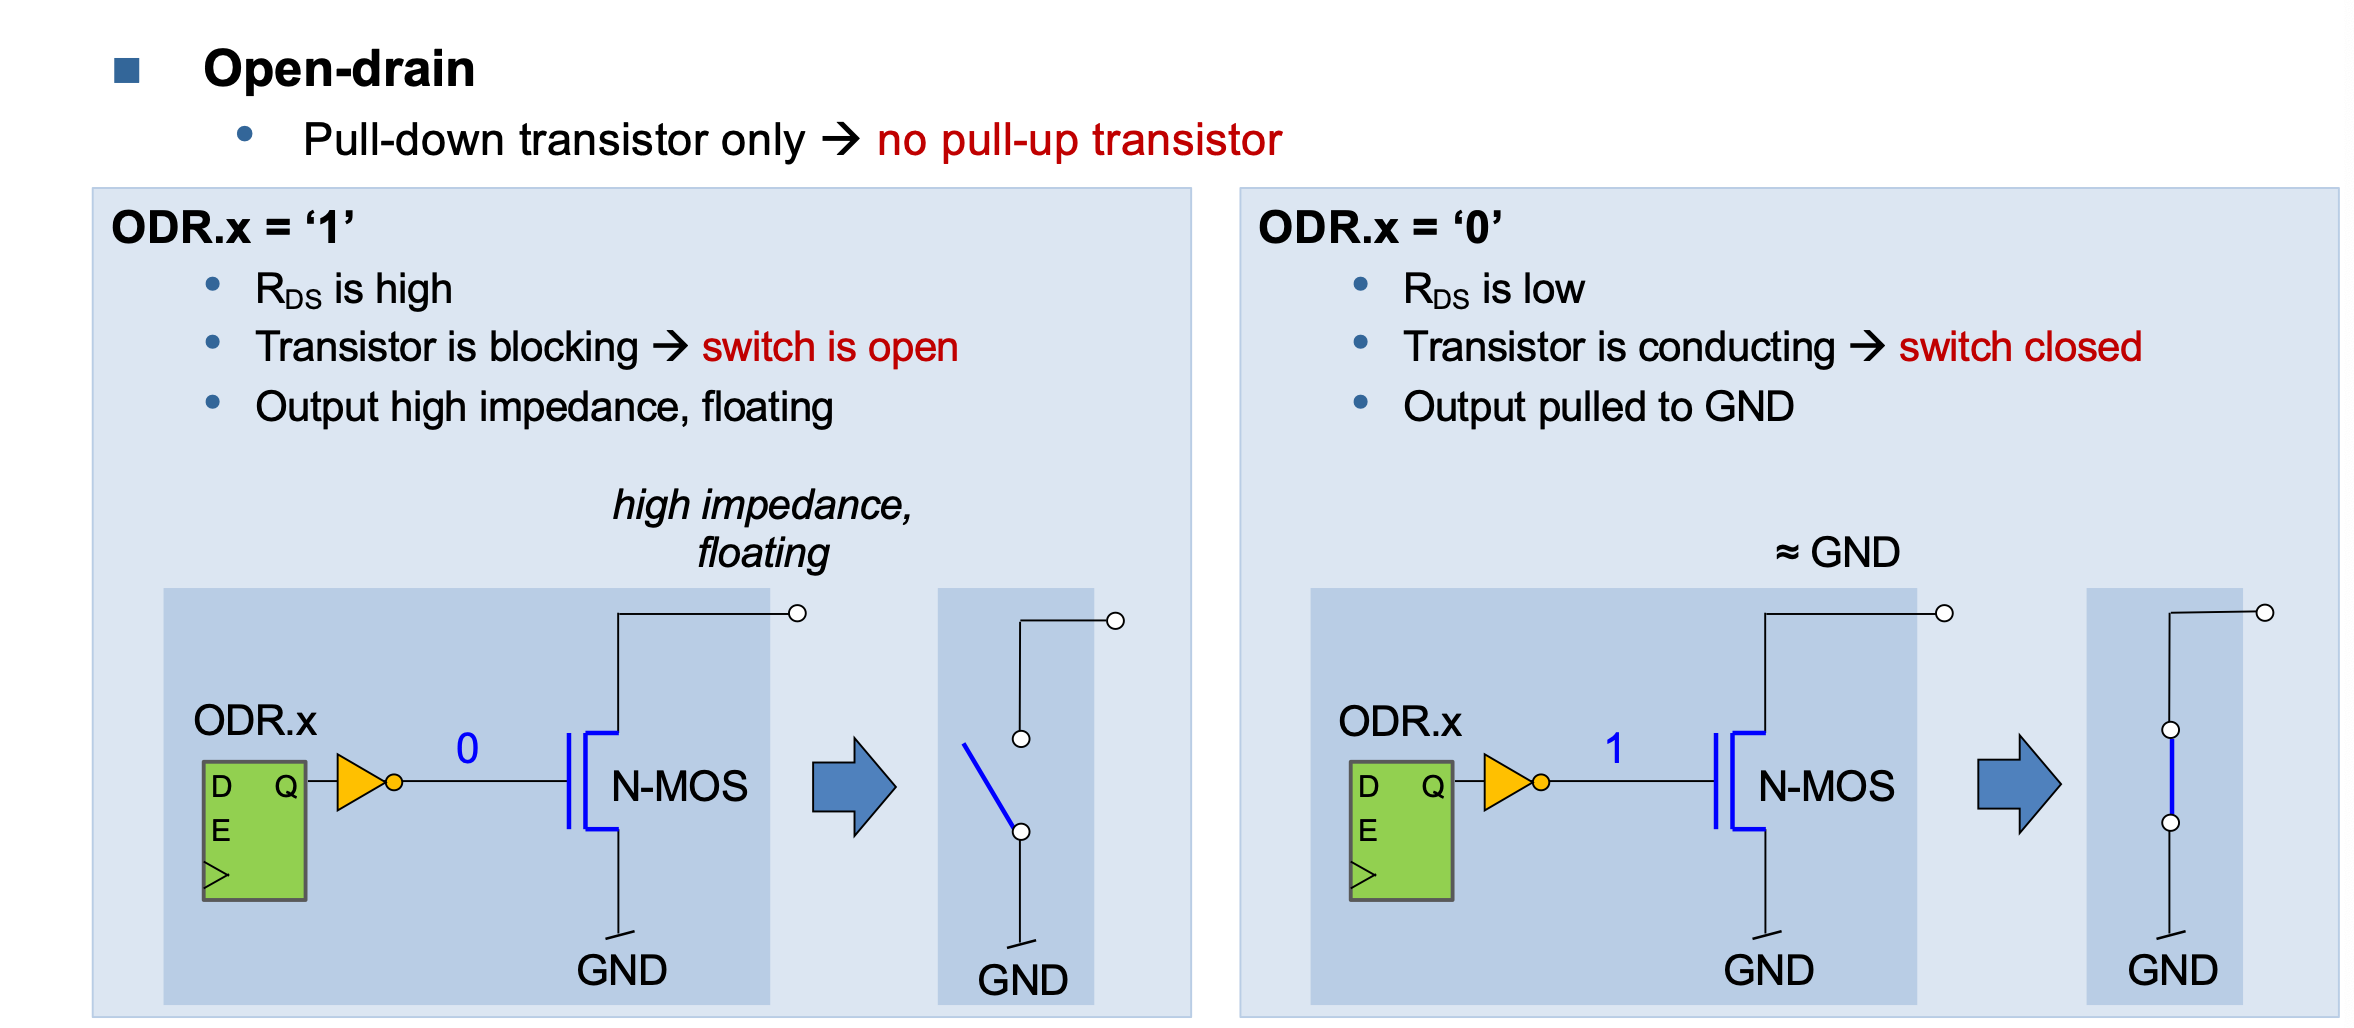
\includegraphics[width=0.3\textwidth]{sections/images/push_pull2.png}
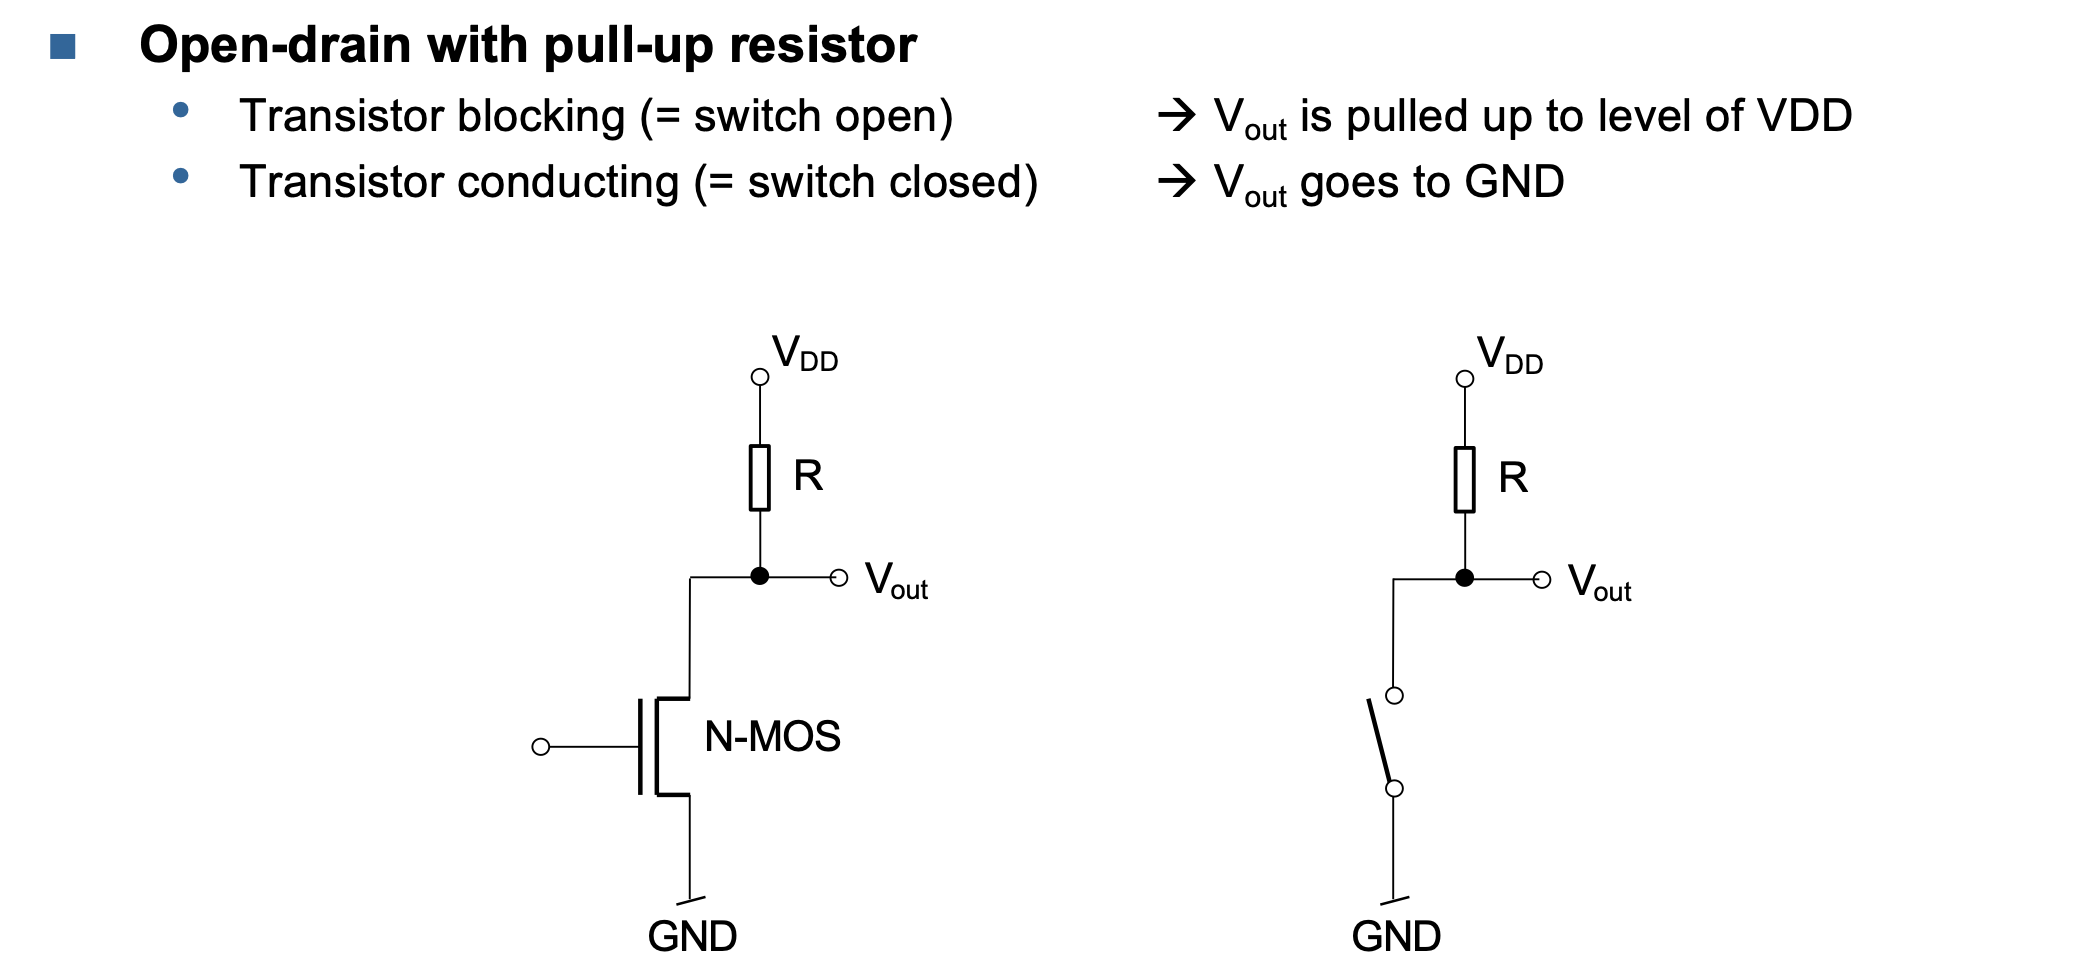
\includegraphics[width=0.3\textwidth]{sections/images/push_pull3.png}

\subsubsection{Pull-up und Pull-down konfigurieren}
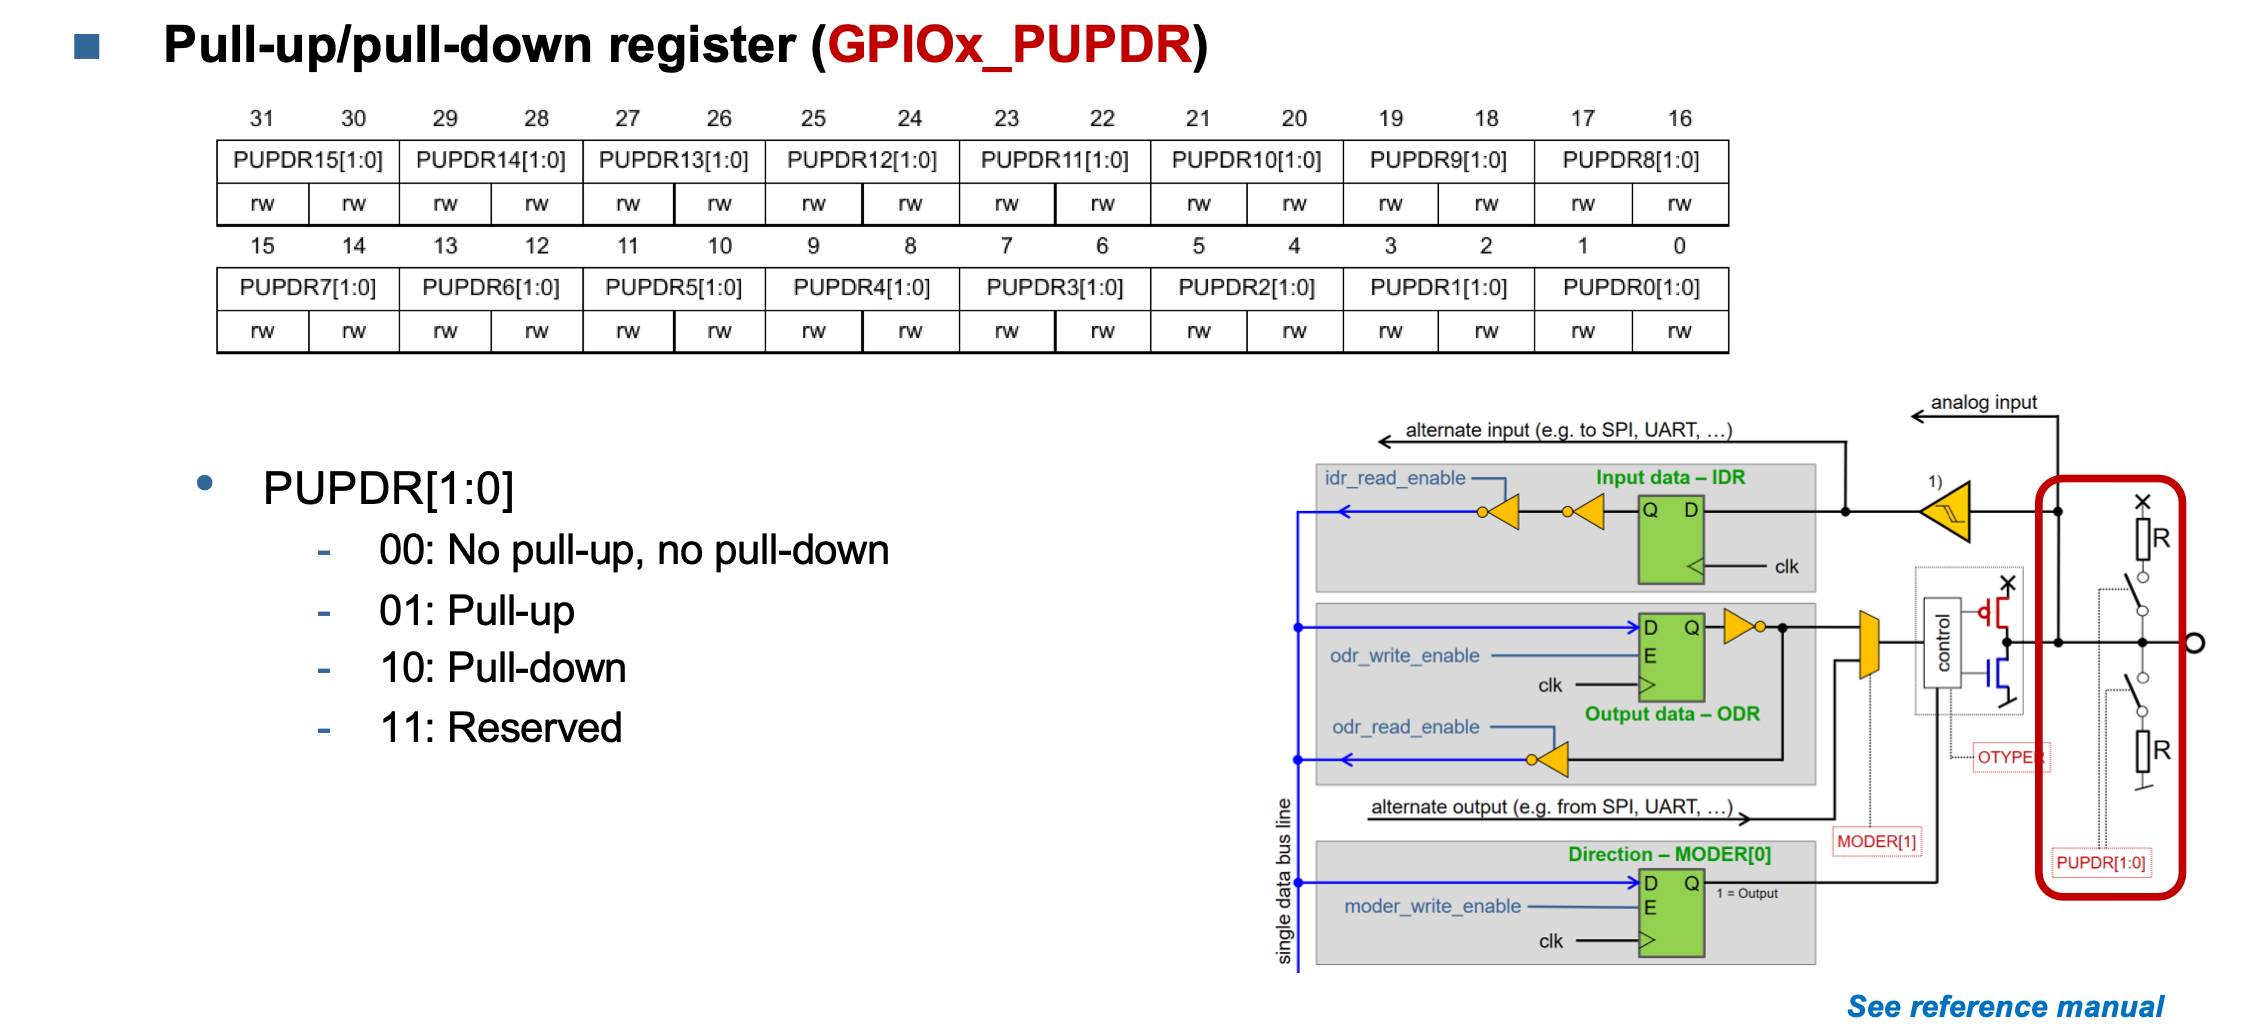
\includegraphics[width=0.3\textwidth]{sections/images/pullup.png}

\subsection{Speed Register}
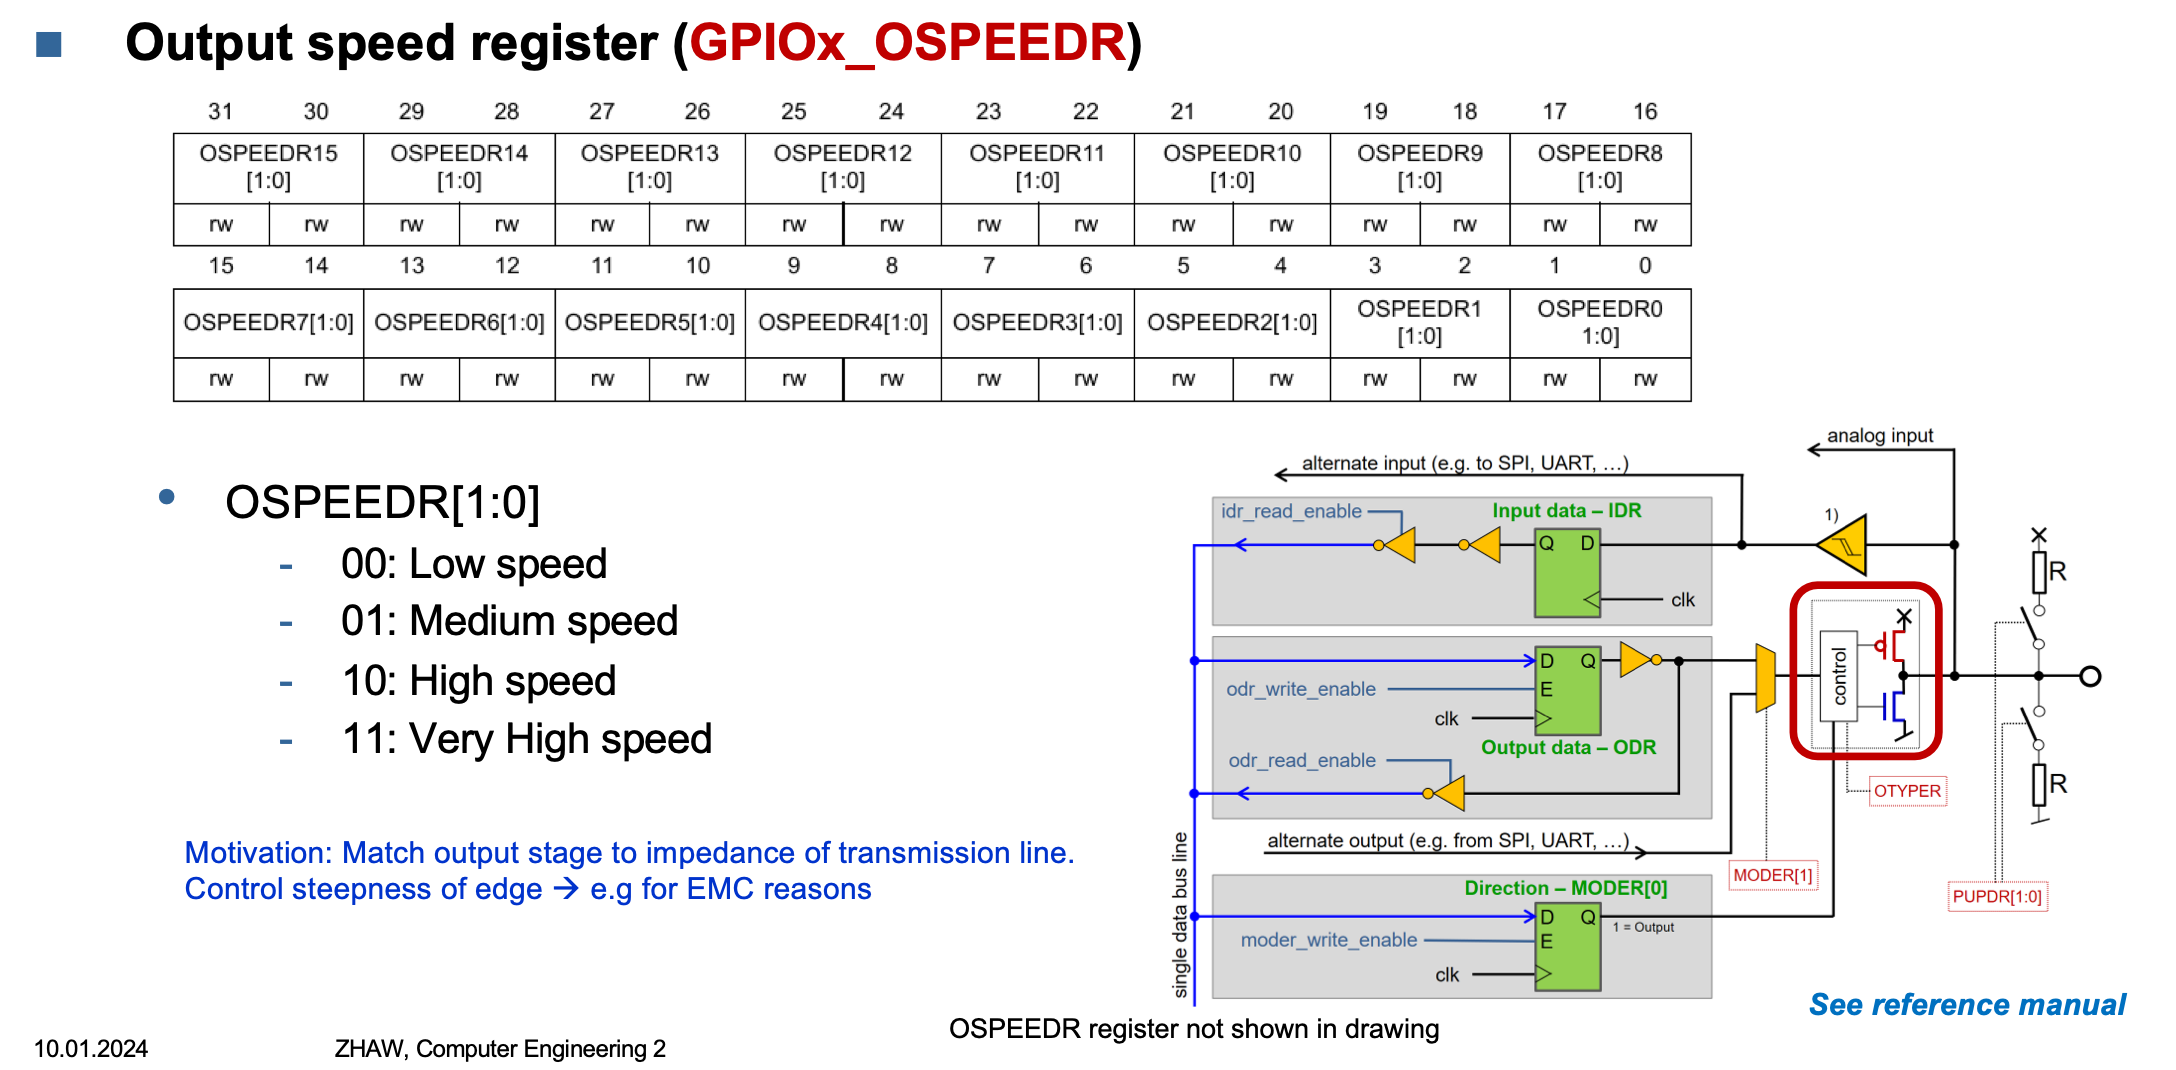
\includegraphics[width=0.3\textwidth]{sections/images/speed.png}

\subsection{I/O Port Konfiguration}
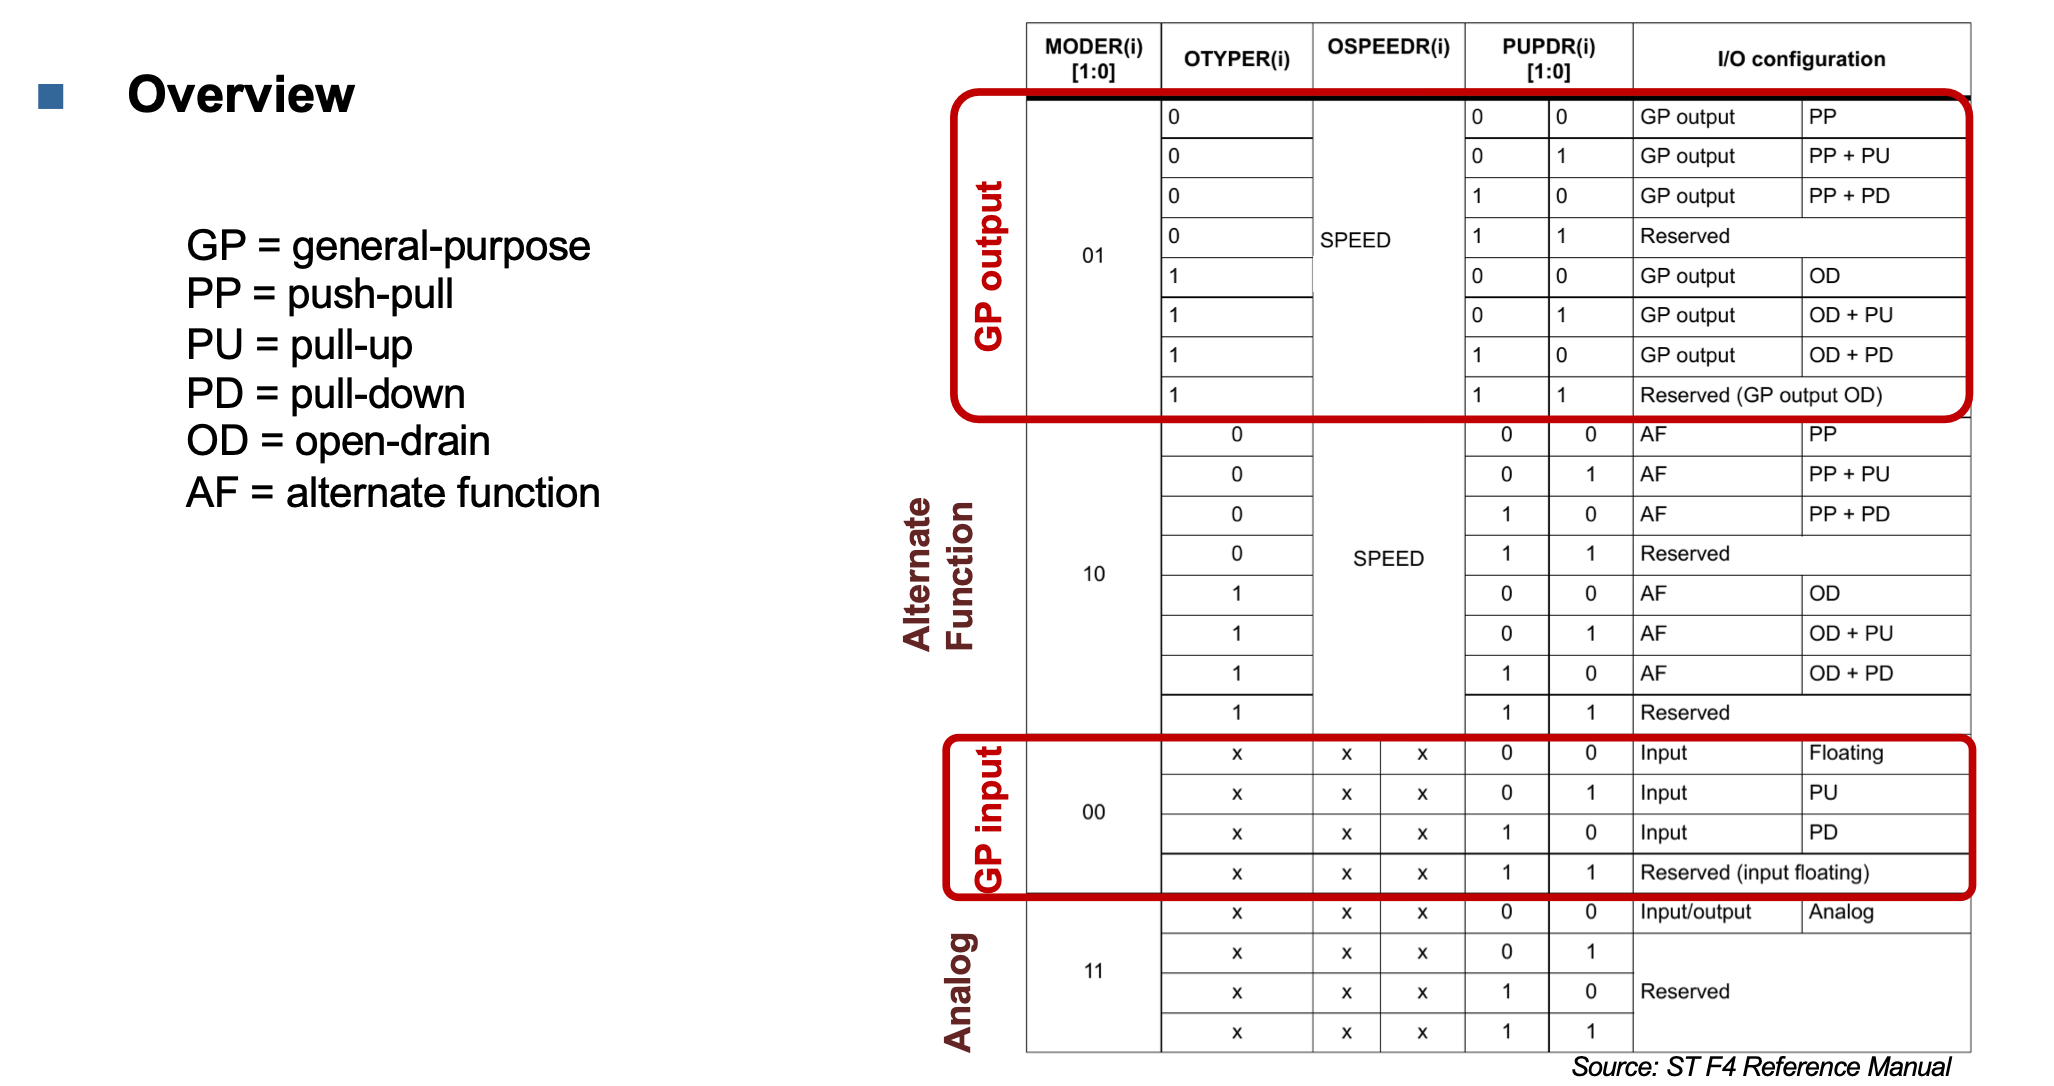
\includegraphics[width=0.3\textwidth]{sections/images/io_config.png}

\subsection{Input lesen}
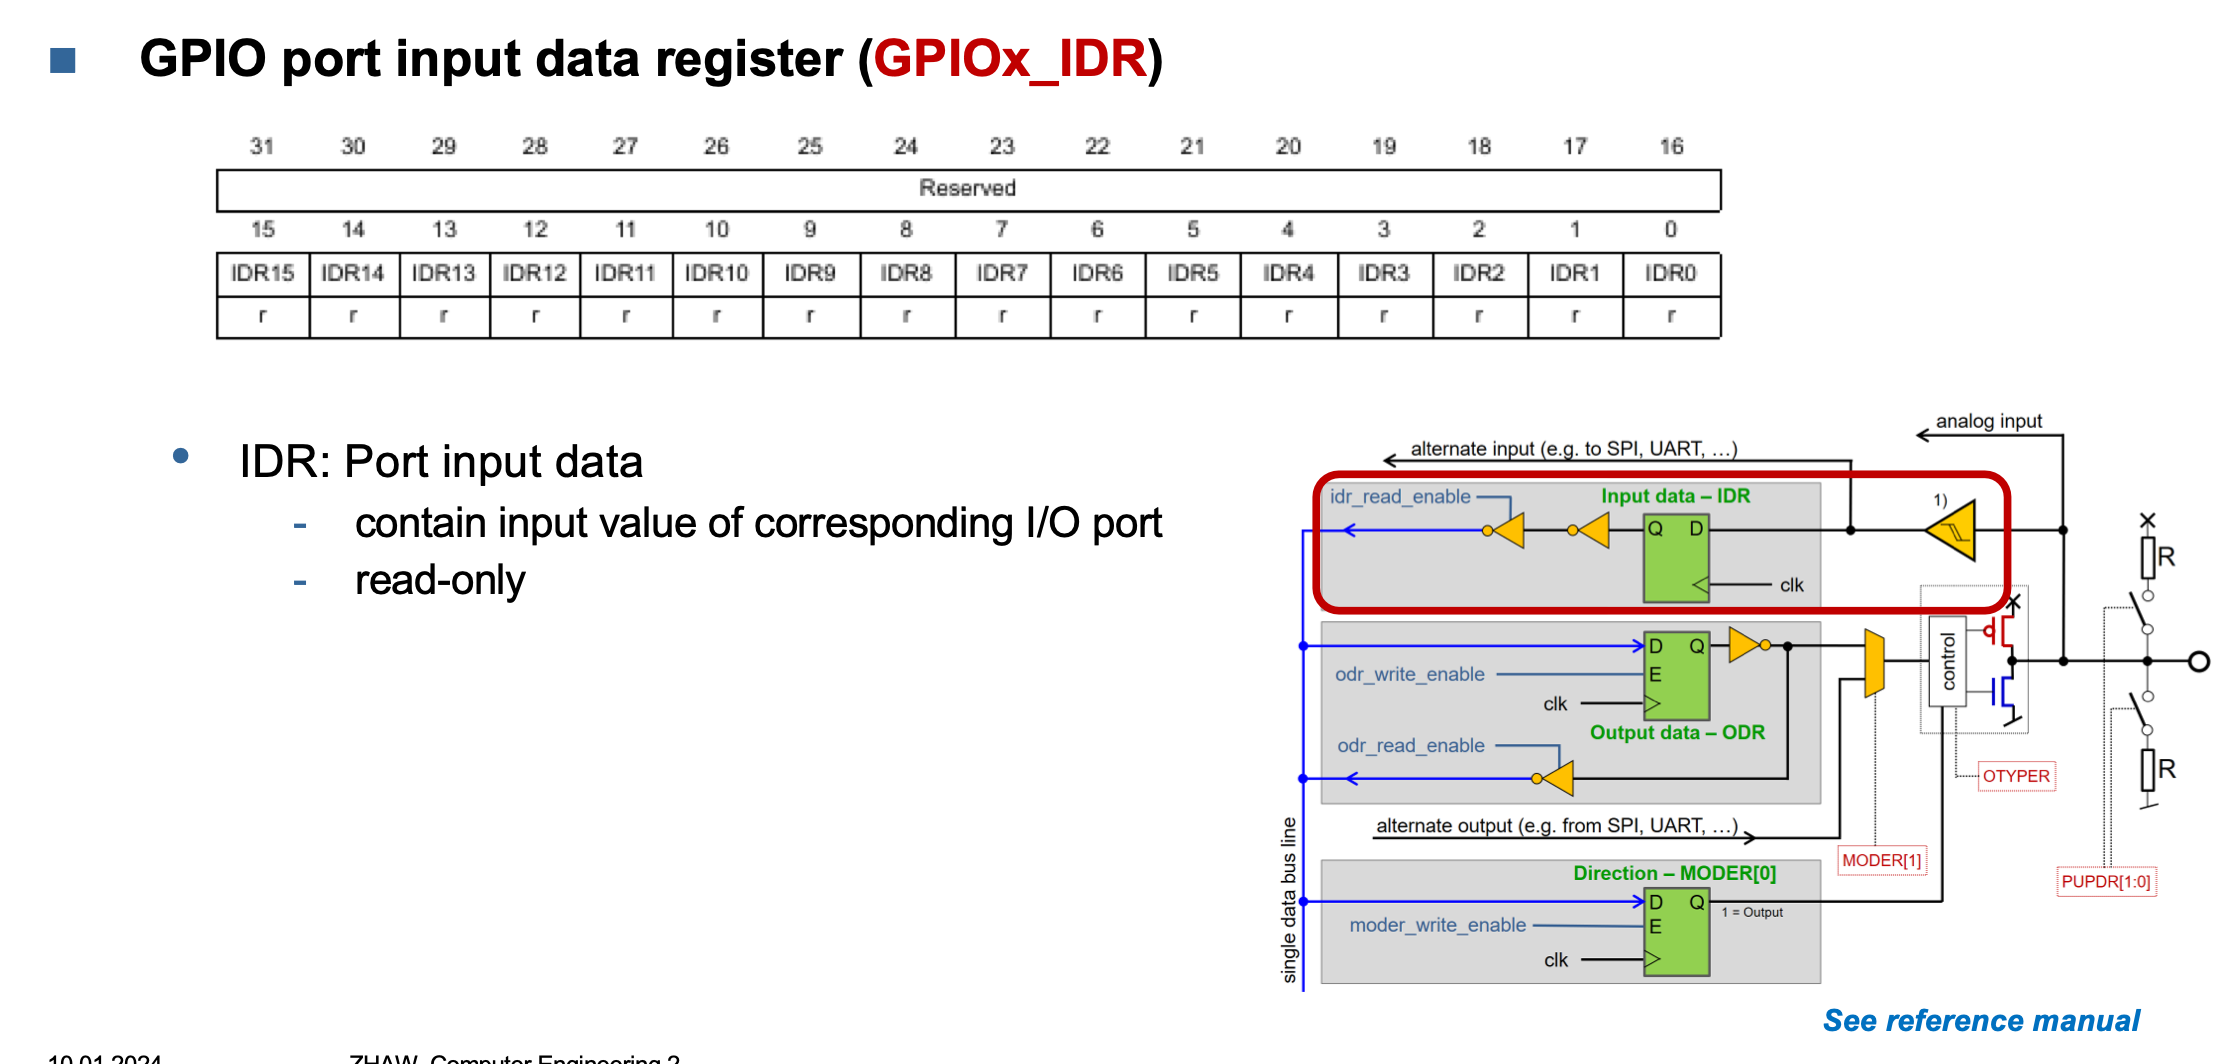
\includegraphics[width=0.3\textwidth]{sections/images/reading_gpio.png}

\subsection{Output schreiben}
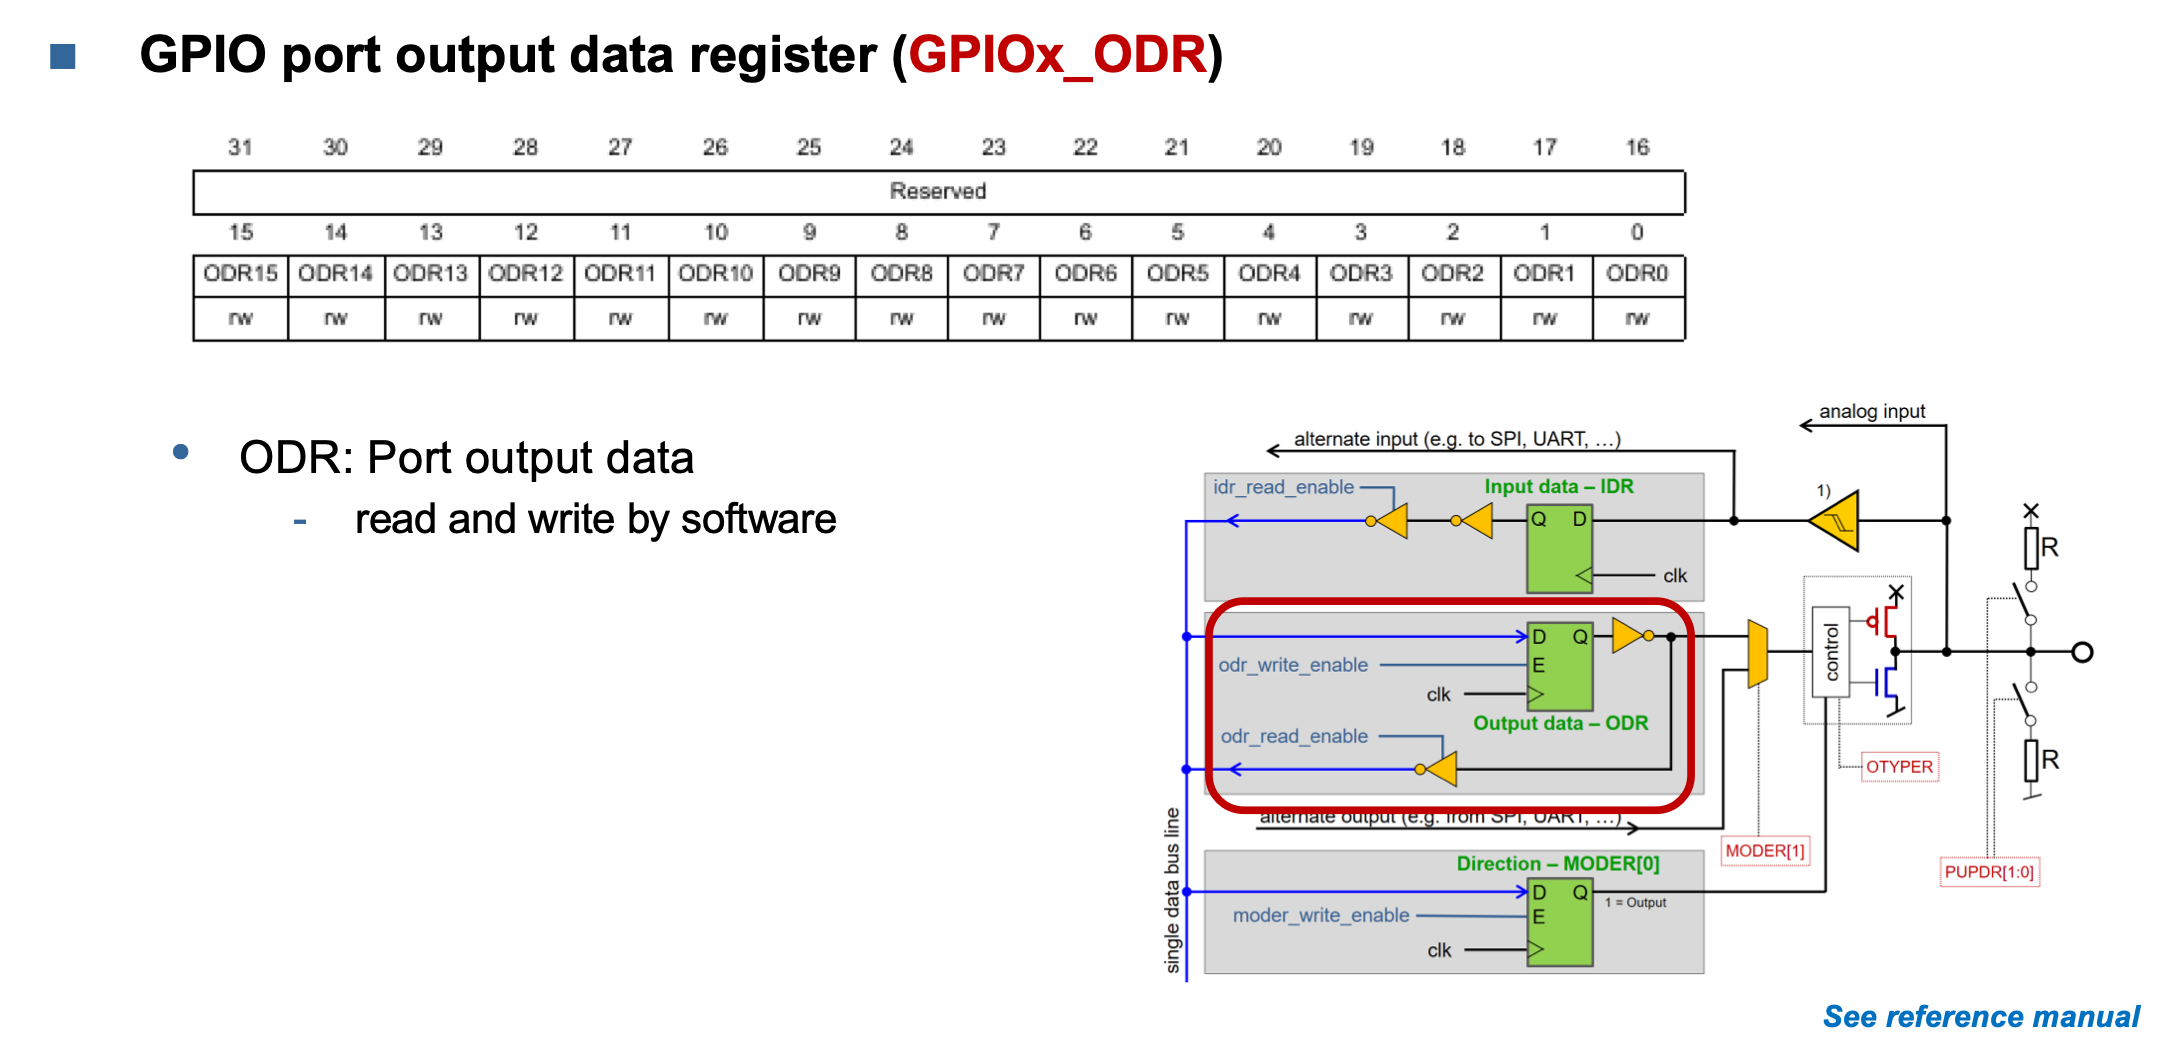
\includegraphics[width=0.3\textwidth]{sections/images/writing_gpio.png}

\subsection{Bits setzen und löschen}
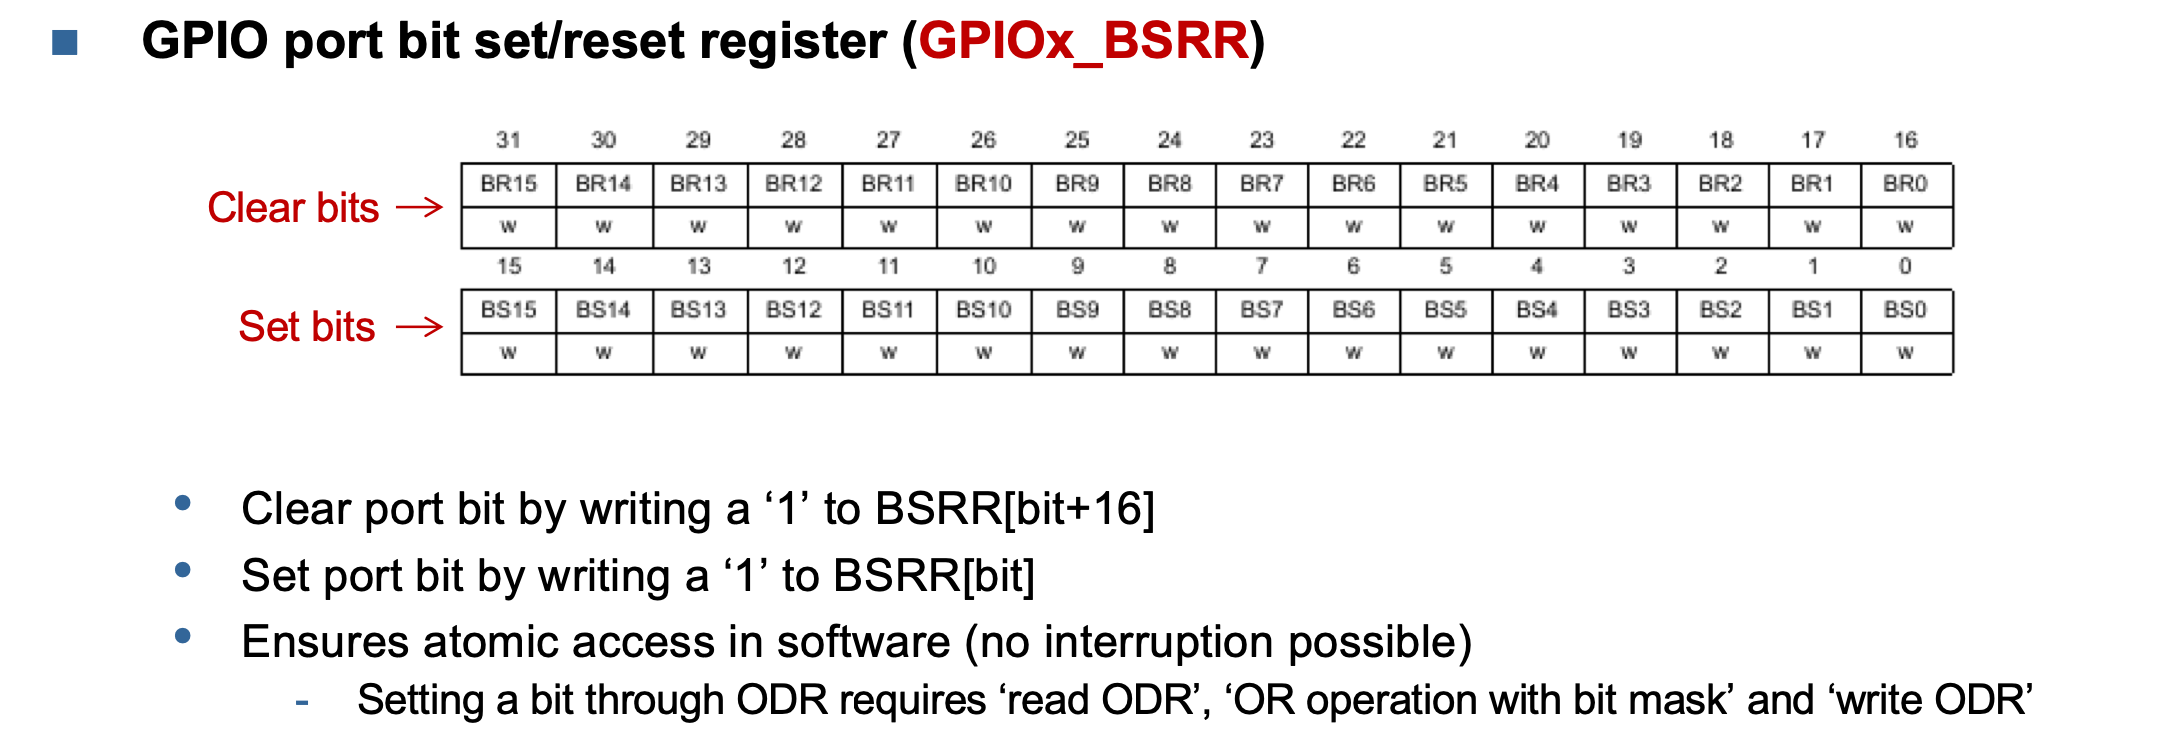
\includegraphics[width=0.3\textwidth]{sections/images/set_gpio.png}

\subsection{GPIO Beispiel}
Auf einem STM32F429 soll Pin 37 als low-speed Output mit open-drain und pull-up konfiguriert werden. Welche Register müssen gesetzt werden? Welche Bits müssen gesetzt werden?

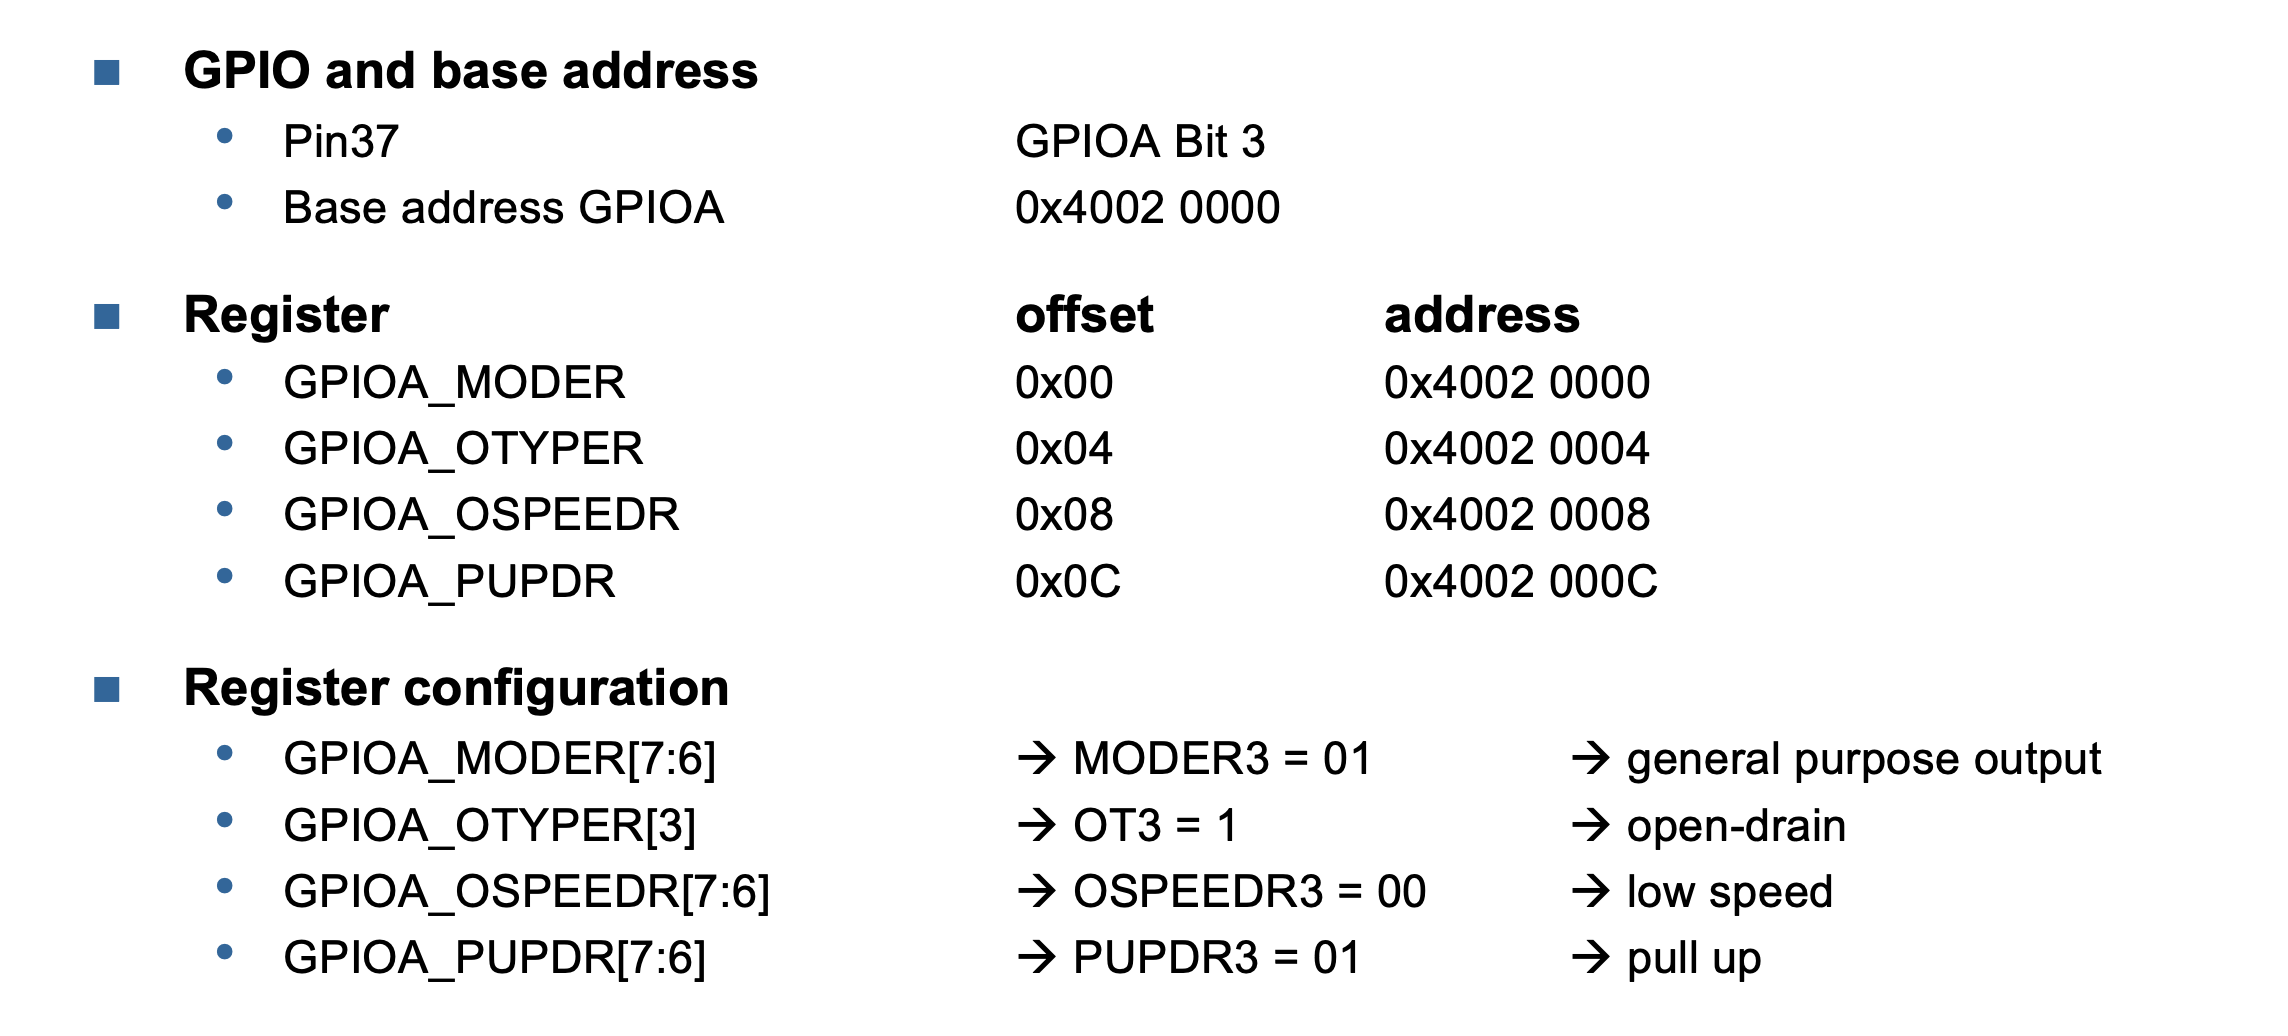
\includegraphics[width=0.3\textwidth]{sections/images/beispiel_gpio.png}

\subsection{Hardware Abstraction Layer (HAL)}
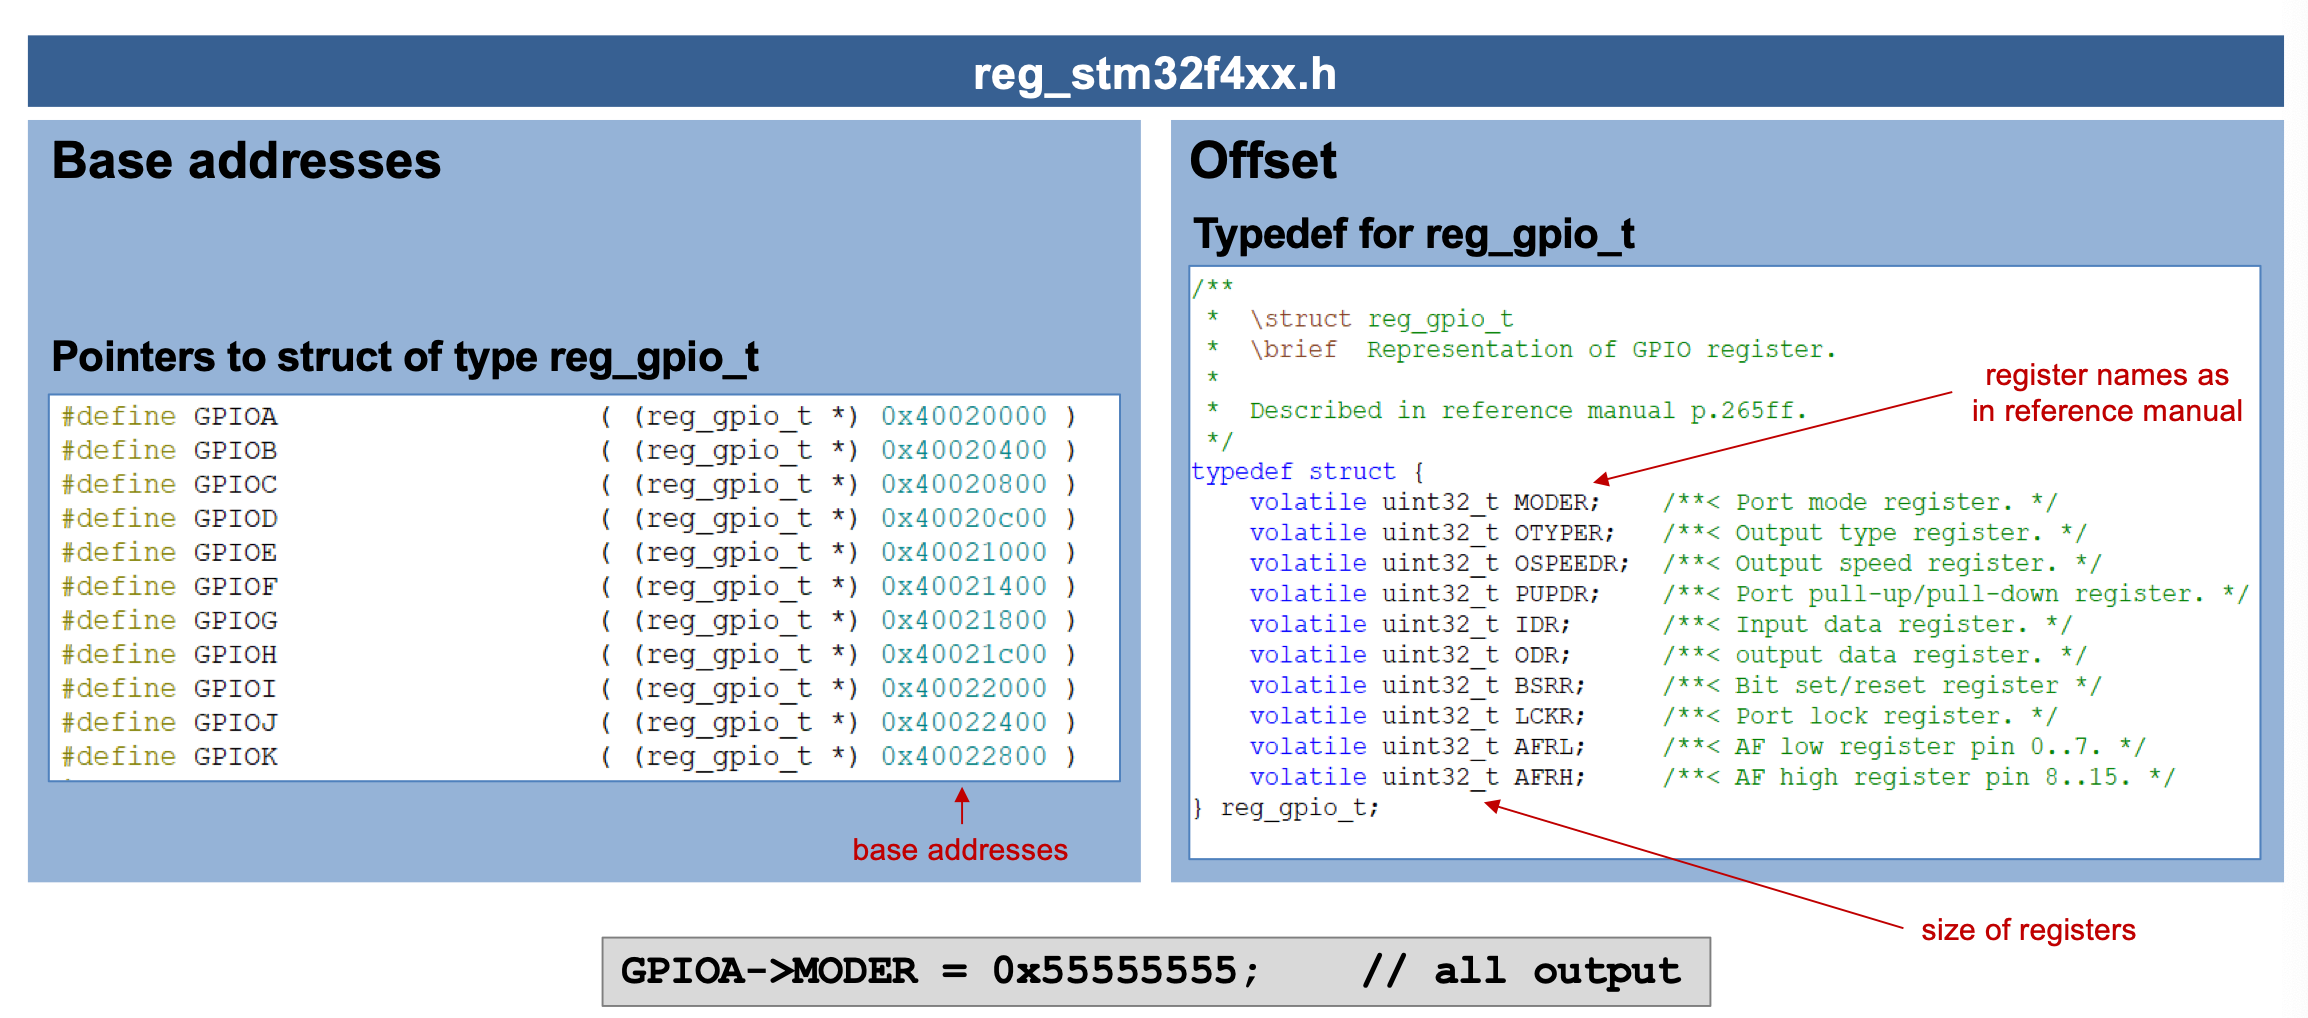
\includegraphics[width=0.3\textwidth]{sections/images/hal.png}

\subsubsection{HAL Beispiel: Code für Konfiguration oben}
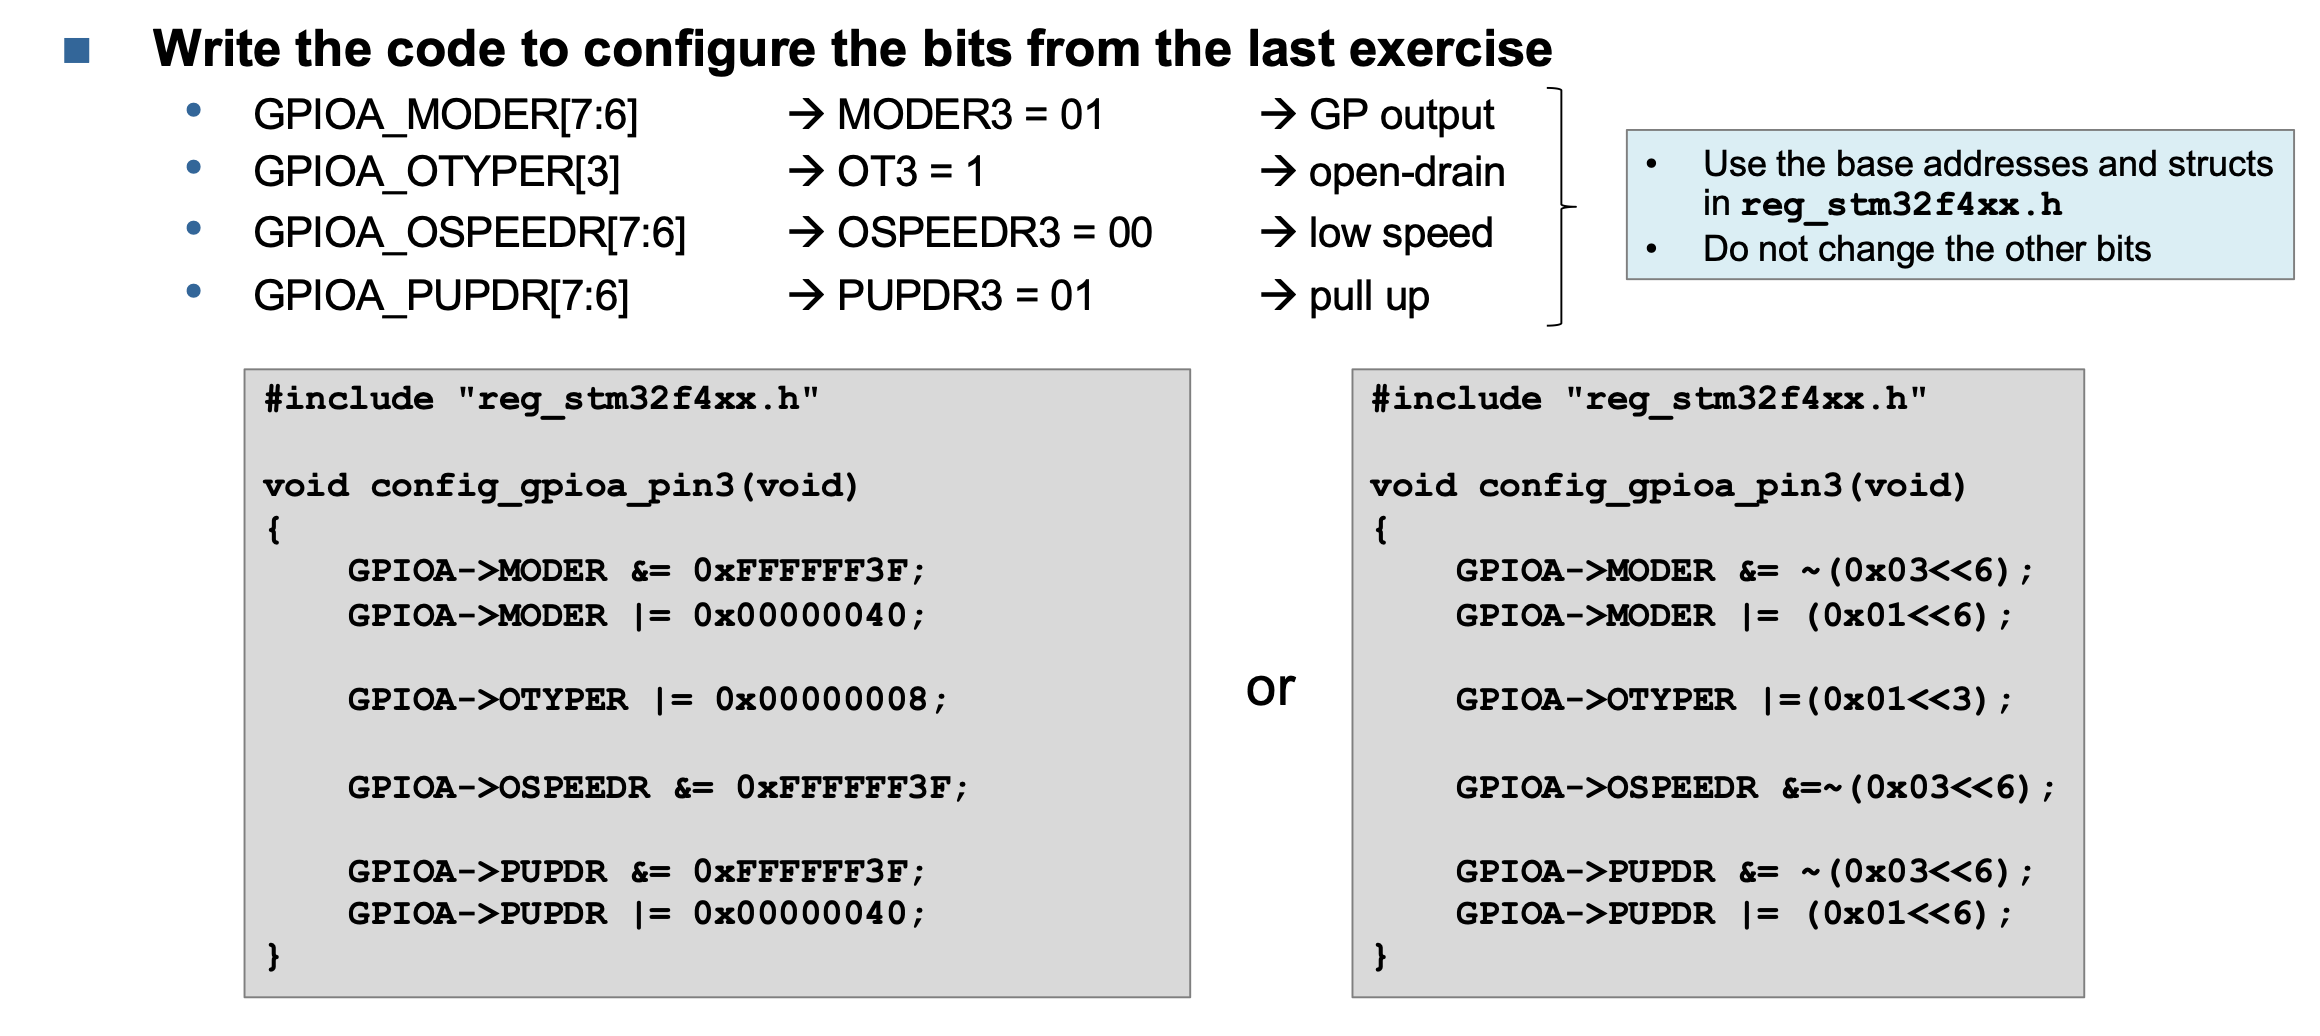
\includegraphics[width=0.3\textwidth]{sections/images/code_gpio_beispiel.png}